%%%%%%%%%%%%%%%%%%%%%%%%%%%%%%%%%%%%%%%%%%%%%%%%%%%%%%%%%%%%%%%%%%%%%%%
%% Vorlage fuer Abschlussarbeit (IFM, FB-T, FH Bielefeld)
%% Autor: Carsten Gips, modified by Matthias Koenig
%% Datum: 04.04.2013
\documentclass[11pt, a4paper]{article}




%%%%%%%%%%%%%%%%%%%%%%%%%%%%%%%%%%%%%%%%%%%%%%%%%%%%%%%%%%%%%%%%%%%%%%%
%% Nuetzliche Pakete
\usepackage{natbib} 
\usepackage[english, ngerman]{babel}
\usepackage[utf8]{inputenc}
\usepackage[T1]{fontenc}
\usepackage{lmodern}   
\usepackage{marvosym}
% \usepackage{times}

\usepackage[babel]{csquotes}
\usepackage[a4paper, left=2.5cm, right=2.5cm, top=2.5cm, bottom=2.5cm]{geometry}
\usepackage{setspace}
% \usepackage{latexsym}
% \usepackage{exscale}
% \usepackage{verbatim}
% 
% \usepackage{tikz}
% \usepackage{wasysym}
\usepackage{graphicx}
\usepackage{subfigure}
\usepackage{listings}
% \usepackage{fancybox}
% \usepackage{pdfpages}
% \usepackage{xspace}
\usepackage{hyperref}
\usepackage{color}
% \usepackage[table]{xcolor}
% \usepackage{colortbl}
% \usepackage{supertabular}
% \usepackage{colortbl}
% \usepackage{rotating}
\usepackage{textcomp}
\usepackage{ dsfont }
\usepackage[ruled,vlined]{algorithm2e}
\usepackage{tabularx}
\usepackage{longtable, tabu}
\usepackage{float}
% 

\usepackage{amssymb,amsmath}

\definecolor{listinggray}{gray}{0.92}
\definecolor{commentgray}{gray}{0.6}
\definecolor{quellengray}{gray}{0.8}

\lstset{language=bash}

\lstnewenvironment{java}{
%\lstset{xleftmargin=\bigskipamount, xrightmargin=\bigskipamount, aboveskip=\bigskipamount, belowskip=\bigskipamount,}
\lstset{language=Java, basicstyle=\footnotesize\ttfamily\mdseries}
\lstset{keywordstyle=\bfseries\color{blue},identifierstyle=\ttfamily, commentstyle=\bfseries\color{gray}\textsl,stringstyle=\color{magenta}\upshape}
\lstset{emphstyle=\color{red}, emphstyle={[2]\color{blue}}}
%\lstset{texcl=true}
\lstset{texcl=false}
\lstset{escapechar=@}
\lstset{inputencoding=utf8}
%\lstset{framexleftmargin=5mm, frame=shadowbox, rulesepcolor=\color{black}}
\lstset{columns=fullflexible, showspaces=false, showstringspaces=false, numbers=none, breaklines=true,tabsize=4, backgroundcolor=\color{listinggray}}
}{}





% \usepackage{makeidx}         % index
% \makeindex
% % damits angezeigt wird:
% % makeindex diss.idx
% \usepackage[german]{nomencl} % nomenclatur
% \makeglossary
% % damits angezeigt wird:
% % makeindex diss.glo -s nomencl.ist -o diss.gls
% 
% \usepackage{theorem}
% \usepackage{varioref}  % \vref{} ...


% % \sloppy




%%%%%%%%%%%%%%%%%%%%%%%%%%%%%%%%%%%%%%%%%%%%%%%%%%%%%%%%%%%%%%%%%%%%%%%
%% Start des Dokuments
\begin{document}
\onehalfspacing







%%%%%%%%%%%%%%%%%%%%%%%%%%%%%%%%%%%%%%%%%%%%%%%%%%%%%%%%%%%%%%%%%%%%%%%
%% Titelseite
%%%%%%%%%%%%%%%%%%%%%%%%%%%%%%%%%%%%%%%%%%%%%%%%%%%%%%%%%%%%%%%%%%%%%%%
%% Titelseite
% \maketitle    % Anzeige der Standardtitelseite
\begin{titlepage}
\thispagestyle{empty}
    \hrule
    \vspace{1cm}
    \begin{center}
      
        {\huge\bf\sc Roboter-Roboter Interaktion zur autonomen Objektübergabe}
    \end{center}
    \vfill
    \begin{Large}
        {\bf Master-Abschlussarbeit},\\[48pt]
        eingereicht am Fachbereich Technik\\
        der FH Bielefeld\\[72pt]
        von Robin Rasch,\\
        geboren am 05.02.1991 in Minden
        \vfill
        \noindent{\today}
    \end{Large}
    \vspace{1cm}
    \hrule
\end{titlepage}


\clearpage


%%%%%%%%%%%%%%%%%%%%%%%%%%%%%%%%%%%%%%%%%%%%%%%%%%%%%%%%%%%%%%%%%%%%%%%
%% Erklaerung
%%%%%%%%%%%%%%%%%%%%%%%%%%%%%%%%%%%%%%%%%%%%%%%%%%%%%%%%%%%%%%%%%%%%%%%
%% Eidesstattliche Erklaerung
\thispagestyle{empty}
{\ }    % sonst wirkt das \vfill nicht
\vfill
\noindent{Mit meiner Unterschrift bestätige ich, dass ich die Arbeit
selbständig und nur mit den zugelassenen Hilfsmitteln erstellt habe.}

\vspace{20mm}

\noindent{Minden, den \dotfill}

    
    \clearpage


%%%%%%%%%%%%%%%%%%%%%%%%%%%%%%%%%%%%%%%%%%%%%%%%%%%%%%%%%%%%%%%%%%%%%%%
%% Abstract
%%%%%%%%%%%%%%%%%%%%%%%%%%%%%%%%%%%%%%%%%%%%%%%%%%%%%%%%%%%%%%%%%%%%%%%
%% Abstract
\begin{abstract}
\thispagestyle{empty}

  Diese Arbeit befasst sich mit der Entwicklung und Implementierung eines autonomen Roboter Systems. Dieses System bildet das Szenario einer Objektübergabe zwischen zwei selbstständigen Manipulatoren ab. Bei diesen beiden Manipulatoren handelt es sich um den Typ-gleichen Roboterarm des YouBot der Firma Kuka. Einer der Arme ist dabei stationär auf einem Tisch fixiert, der andere auf der mobilen YouBot Plattform.
  
  Nach einer kurzen Einführung über das Nutzen von Robotern im Haushalt, sowie im intelligenten Gebäude, werden zunächst die Grundlagen und folgend ein aktueller Stand der Technik zusammengefasst. Anschließend wird sich diese Arbeit mit den zentralen Aspekten der Entwicklung und Implementierung befassen. Bei der Entwicklung wurden verschiedene Thematiken und Probleme der Robotik und Computer Vision berücksichtigt und bearbeitet. So werden die folgenden Kapiteln auf das Setup der Roboter eingehen, sowie den Themen der inversen Kinematik, der Segmentierung und Objekterkennung. Da das System in einem intelligenten Gebäude zum Einsatz kommen soll, ist die Thematik der Konfigurierung einzelner Subsysteme und Koordination ein Bestandteil dieser Arbeit. Die Implementierung befasst sich mit der Algorithmik der einzelnen Probleme. Den Abschluss der Arbeit bilden eine Beurteilung und ein Fazit der umgesetzten Lösung, auch wird ein Ausblick über mögliche zukünftige Weiterentwicklungen gegeben.
  
\end{abstract}




\begin{otherlanguage}{english}
	\begin{abstract}
		This paper considers the development and implementation of an autonomous robotic system. This system describes a scenario from a handover between two independent manipulators. These two manipulators are equal robot arms from the Kuka YouBot. One is stationary fixed at top of a table, the other one is on a mobile YouBot base.
		
		After a short introduction about the harness of service robots at smart houses, this work outlines the principles and the state of the art. Following this paper attends to the key aspects of the development and the implementation. The development observes different topics and a set of problems for robotic and computer vision. There will be a variety of subjects like roboter setup, inverse kinematic, segmentation and object recognition in the following chapters. Based on the operation at smart houses,  are konfiguration and koordinaten topics in this paper, too. The implementation sink in algorithmic and solutions for single problems. A valutation and a conclusion of the implemented solutions, and also a prospect of possible future projects, form the ending of this work. 
	\end{abstract}

\end{otherlanguage}


\clearpage


%%%%%%%%%%%%%%%%%%%%%%%%%%%%%%%%%%%%%%%%%%%%%%%%%%%%%%%%%%%%%%%%%%%%%%%
%% Verzeichnisse
\input{tex/verzeichnisse}\clearpage





%%%%%%%%%%%%%%%%%%%%%%%%%%%%%%%%%%%%%%%%%%%%%%%%%%%%%%%%%%%%%%%%%%%%%%%
%% Einleitung
%%%%%%%%%%%%%%%%%%%%%%%%%%%%%%%%%%%%%%%%%%%%%%%%%%%%%%%%%%%%%%%%%%%%%%%
%% Einleitung
\section{Einleitung}
\label{sec:einleitung}

Der demographische Wandel stellt die Gesellschaft und die Politik vor ein großes Problem. Nicht nur der fehlende Nachwuchs, der ein Arbeitnehmermangel hinterlässt, sondern auch eine immer älter werdende Gesellschaft stellen Schwierigkeiten dar. Neben kommunalen Problemen, wie teure Infrastruktur, ist die Altersarmut eins der größten Anliegen. Ein sinkendes Rentenniveau und steigende Kosten werden es in Zukunft unmöglich machen für eine gute Pflegeversorgung zu bezahlen  \citep{brunozandonella2013}. Neben den hohen Kosten in der Pflege gibt es auch weitere Faktoren, die zu einer nicht akzeptablen Situation führen. So ist der Pflegeberuf zu unattraktiv für viele junge Menschen, wodurch auch hier ein großes Loch an Arbeitnehmern wahrzunehmen ist. Außerdem führt körperlich anstrengende Arbeit, die in kurzer Zeit ausgeführt werden muss, zu vielen physischen und psychischen Erkrankungen der Pfleger \citep{AOK2004}.

Eine mögliche Lösung liegt in der Technik. Einfach zu bedienende Systeme können den Alltag vereinfachen und so auch älteren Menschen ein selbstständiges Leben ermöglichen. Alltägliche Aufgaben müssten nicht mehr von Pflegekräften übernommen werden, sondern könnten durch Maschinen erledigt werden. Schon heute können einzelne Kleinsysteme Haustätigkeiten, wie Staubsaugen und Rasenmähen, übernehmen. Ein Vorreiter auf diesem Gebiet ist das Roboterland Japan. Dort überlegte sich Kobayashi Hisato, Professor für Maschinenbau und Robotik an der Hosei-Universität in Tokio, schon 1999 Konzepte für Senioren-Service-Roboter \citep{wagner2009tele}. Nach seinen Vorstellungen sollten dabei Roboter nicht autonom arbeiten, sondern von Familienangehörigen ferngesteuert und überwacht werden \citep{kobayashihisato1999}. Neben diesen Konzepten kann man aber auch schon angewandte Robotik in Japans Seniorenpolitik finden. Zwei Musterbeispiele zeigen dabei die unterschiedlichen Anwendungsszenarien für Roboter im privaten Umfeld. \textit{Sinére K\={o}rien} der Firma Matsushita ist ein digitales Seniorenheim. Neben einer Smarthouse Anbindung gehört auch der Roboterteddy K\={o}-chan zur Ausstattung der einzelnen Zimmer (siehe Abbildung \ref{fig:roboTeddy}). Dieser dient als Unterhaltungsroboter und Kommunikationsgerät mit den Pflegerkräften. So kann mit den Kameraaugen im Teddy eine Aufnahme vom Raum gemacht werden und im Notfall den Pflegekräften eine Alarmmeldung geschickt werden. Weitere Sensoren, zum  Beispiel Gewichtssensoren unter den Betten, geben Informationen über die Abwesenheiten von Patienten \citep{wagner2009tele}. Ein weiterer Anwendungsbereich für Roboter ist die \textit{robotto serap\={\i}} (Robotertherapie). Dabei beschäftigen sich Senioren mit tierähnlichen Robotern, wie Hunden, Seerobben oder Katzen (siehe Abbildung \ref{fig:roboTeddy2}). Im Zentrum der Therapie steht die Interaktion zwischen Patient und Roboter. Die Robotertherapie soll die Patienten aktivieren und deren Tagesabläufe abwechslungsreich gestalten. Außerdem steigert es die Kommunikation zwischen zwei Patienten, die am selben Roboter arbeiten \citep{wagner2009tele}. 

 \begin{figure}
 	\centering
 	\subfigure[Roboterteddy K\={o}-chan. Bildquelle: \citep{panasonic2005}]{%
 		\includegraphics[scale=0.6]{fig/roboteddy}
 		\label{fig:roboTeddy}}
 	\hfill
 	\subfigure[Roboterkatze zur Therapie. Bildquelle: \citep{wagner2009tele}]{%
 		\includegraphics[scale=0.4]{fig/robocat}
 		\label{fig:roboTeddy2}}
 	\caption{Roboter in Seniorenheimen}
 	\label{fig:robSenioren}
 \end{figure}

Nicht nur in Japan, sondern auch in Deutschland wird sich mit dem Thema \textit{Care(rob)bots} befasst. So finden sich unter dem Stichpunkt \textit{Mensch-Maschine-Entgrenzungen} Studien zu der Thematik. Andere Untersuchungen befassen sich mit der Gegenseite, der Akzeptanz der Senioren für Roboter. So ergab eine Befragung der VDE-Studie "Mein Freund der Roboter", dass eine Mehrheit (56\%) der Senioren Robotern im Haushalt offen gegenüber stehen und diese einem Pflege-/Altersheim vorziehen würden. Neben den bekannten Staubsauger- und Rasenmährobotern, sind es auch zukünftige Anwendung, wie ein roboterisierter Rollstuhl, die hohe Akzeptanzwerte erreichen. Die Studie zeigte aber auch, dass Senioren zunächst Robotern skeptisch gegenüberstehen. Spontan lehnten 40 Prozent der Senioren Roboter in ihrem privaten Umfeld ab, 60 Prozent empfanden Robotik sogar als unheimlich. Jedoch zeigte sich, dass der Wunsch nach einer selbstständigen Lebensführung ein starker Faktor für die Akzeptanz ist. Dadurch ergibt sich eine Beliebtheit für Serviceroboter. So sind Roboter sehr beliebt, die abgrenzbare Tätigkeiten im Haushalt selbständig erledigen. Wichtige Kriterien für die Akzeptanz waren zudem die intuitive Bedienbarkeit, die Robustheit und die Flexibilität gegenüber unterschiedlicher Handicaps. Auch menschliche Faktoren wie Geduld, Verständnis, Höflichkeit und Achtung der Intimsphäre waren den Anwendern wichtig \citep{dr.sibyllemeyer2011}.

Neben den sozialen Forschungen gibt es in Deutschland auch ingenieurwissenschaftliche Ergebnisse auf diesem Gebiet. So beschäftigt sich das Cluster of Excellence Cognitive Interaction Technology (CITEC) in Bielefeld, zusammen mit der Stiftung Bethel, in der Forschung auf dem Gebiet der Unterstützung für Demenzkranke. Die dort entwickelten Assistenzsysteme helfen den Patienten unter anderem beim Zähneputzen und geben ihnen so ein Stück Selbstständigkeit zurück \citep{peters2010task}. 

Viele Forschungen und Entwicklungen beschäftigen sich momentan mit der Mensch-Maschine/ -Roboter Beziehung. Dabei geraten die Roboter-Roboter-Interaktionen in den Hintergrund. Heutige Roboter sind keine Allround-Lösungen, sondern meist hochgradig spezialisiert und nur eine Tätigkeit ausführen können (zum Beispiel Saugroboter, Fensterwischroboter und weitere). Deshalb ist die Konfiguration und Koordinierung der Roboter wichtig. Das Szenario in Abbildung \ref{fig:szen1} zeigt, wie solch ein Multi-Robot System aussehen könnte.

\begin{figure}
	\centering
	\includegraphics[width=\textwidth]{fig/szen1}   
	\caption[Beispiel Szenario 1]{Mensch A stößt einen Blumentopf um (1). Ein Kamerasystem detektiert, dass der Topf umgefallen ist und Erde auf dem Boden liegt. Ein Roboter mit Arm wird gerufen, der zunächst die Vase aufhebt und an ihren Platz zurückstellt (2). Anschließend wird ein Saugroboter aktiviert, der die Erde wegsaugt (3). Bei schwereren Verschmutzungen wird noch ein Wischroboter bestellt.}
	\label{fig:szen1}
\end{figure}

Dabei führt jeder Agent selbstständig  und unabhängig von den anderen seine Arbeit aus. Die Koordinierung geht immer von der zentralen Steuereinheit aus. Zwischen den einzelnen Robotern findet kein Informationsaustausch statt. Die Agenten arbeiten seriell ihre Aufgaben ab. Die Änderung an dem Szenario in Abbildung \ref{fig:szen2} ändert jedoch die Art der Koordinierung. Dadurch wird ein Informationsaustausch zwischen den einzelnen Robotersystemen nötig. Auch paralleles Arbeiten der Roboter ist dadurch möglich.

\begin{figure}
	\centering
	\includegraphics[width=\textwidth]{fig/szen2}   
	\caption[Erweiterung Szenario 1]{Beim Zurückstellen der Vase stellt der Roboter fest, dass er die gewünschte Position nicht erreichen kann(1), weil sein Arm zu kurz ist. Da auf der Anrichte noch ein weiterer Arm steht, nimmt er die Kommunikation mit diesem Agenten auf. Sie kommunizieren einen Übergabepunkt und führen ein Übergabemanöver durch. Arm 2 stellt nun die Vase an die gewünschte Position.
	}
	\label{fig:szen2}
\end{figure}


Der zentrale Aspekt dieser Arbeit befasst sich mit dem Aufbau eines Multi-Robot-Systems, kurz MRS. Das Anwendungsszenario ist eine Abstraktion von Szenario 2. Roboter 1 übergibt ein Objekt an Roboter 2. Dabei werden verschiedene Thematiken der Robotik aufgegriffen, untersucht und erläutert. Kapitel \ref{sec:basics} befasst sich mit den Grundlagen auf denen diese Arbeit aufbaut. Neben der Nomenklatur wird die Middleware \textbf{R}obot \textbf{O}perating \textbf{S}ystem, kurz ROS, erläutert. Dabei wird auf den Aufbau, sowie die Kommunikationsschicht von Robotersystemen eingegangen. Anschließend folgt eine kurze Einführung in die mechanischen Grundlagen. Dabei werden die Begriffe rund um die Kinematik erklärt. 

In Kapitel \ref{sec:relatedwork} folgt eine detaillierte Übersicht der zugehörigen Literatur. Zunächst werden Arbeiten um das Thema MRS untersucht. Zentraler Aspekt dieser Thematik ist die Koordinierung von mehreren Robotersystemen. Drauf aufbauend wird das PEIS-Konzept erläutert. In diesem wird eine Nutzung von externen Sensoren für MRS gezeigt. Abschließend wird ein kurzer Einblick in Arbeiten zum Thema Greifen und Übergeben gegeben.

Das anschließende Kapitel \ref{sec:basic-aufbau} beschreibt den Aufbau des Teststandes, sowie die verwendete Hardware. Dabei wird auf die einzelne Sensoren und Aktoren eingegangen. Außerdem werden verschiedene Tests mit Prototypen durchgeführt, um die Genauigkeit und Qualität der Ergebnisse einzuschätzen.

Im Kapitel \ref{sec:entwicklung} werden die zentralen Aspekte dieser Arbeit beschrieben. Nach einer Auflistung von Nicht-Funktionalen Anforderungen, die bei der Entwicklung des MRS berücksichtigt werden sollen, werden einzelne Funktionalitäten des MRS entwickelt. Dabei werden Konzepte und Methoden vorgestellt. Anschließend folgt die Vorstellung der einzelnen Agenten, die für das Szenario benötigt werden. Diesen werden die Funktionalitäten und die Hardware zugewiesen. Diese Agenten werden durch das RATS miteinander verbunden. Diese Architektur bildet eine Schlüsselkomponente dieser Arbeit ab. Aufgabe von RATS ist die Zuweisung und Koordinierung von Aufgaben für unabhängigen Agenten. Diese Agenten können Sensoren, Aktoren oder Roboter sein. Anschließend wird die Entwicklung und Umsetzung einer geometrischen inversen Kinematik beschrieben. Diese ist für eine präzise Steuerung des Arms wichtig. Folgend wird in Kapitel \ref{sec:impl} die Umsetzung der Konzepte aus dem vorherigen Kapitel erläutert. Dazu werden die Algorithmen für verschiedene Funktionalitäten kurz dargestellt. Dabei werden Verfahren der Computer Vision und der Robotik angewandt. 

Zum Ende der Arbeit wird zunächst das entwickelte System in Kapitel \ref{sec:test} getestet und die Ergebnisse bewertet. Dabei wird sowohl auf funktionale, wie auch nicht-funktionale Anforderungen, eingegangen. Außerdem werden Problemstellen gesucht und analysiert, damit in Kapitel \ref{sec:end} im Ausblick Verbesserungsmaßnahmen vorgestellt werden können. Zuvor erfolgt jedoch eine Zusammenfassung der Arbeit. In dieser wird auf die Ergebnisse der Arbeit zurückgeblickt.



\clearpage


%%%%%%%%%%%%%%%%%%%%%%%%%%%%%%%%%%%%%%%%%%%%%%%%%%%%%%%%%%%%%%%%%%%%%%%
%% Grundlagen
%%%%%%%%%%%%%%%%%%%%%%%%%%%%%%%%%%%%%%%%%%%%%%%%%%%%%%%%%%%%%%%%%%%%%%%
%% Related Work
\section{Grundlagen}
\label{sec:basics}

Dieses Kapitel befasst sich mit den Grundlagen für die folgenden Kapitel. Es soll dem geneigten Leser Informationen zum Verständnis der Arbeit geben. Die anschließenden Unterkapitel beschreiben zunächst die verwendeten Mathematischen Ausdrücke und Bezeichner um die Lesbarkeit der späteren Formeln zu erleichtern. Nachfolgend wird die Middleware ROS genauer erläutert und unterschiedliche Funktionen sowie Einschränkungen aufgezeigt, die Auswirkungen auf die entwickelte Softwarearchitektur hatten. Darauf folgt eine Definition des Begriffs der Kinematik, welcher im späteren Verlauf der Arbeit für die Entwicklung der inversen Kinematik benötigt wird. Das abschließende Unterkapitel beschreibt die verwendete Hardware und den Laboraufbau im Detail. Weitere Informationen bezüglich der Robotik und grundlegender Mathematischer Begriffe sind im Buch "Robotics, Vision and Control" von Peter Corke zu entnehmen.

%%%%%%%%%%%%%%%%%%%%%%%%%%%%%%%%%%%%%%%%%%%%%%%%%%%%%%%%%%%%%%%%%%%%%%%
%% Related Work
\subsection{Nomenklatur}
\label{sec:basic-math}
    
  Die folgende Tabelle erläutert die genutzten mathematischen Symbole und orientiert sich an dem Buch "Robitcs, Vision and Control". Von links nach rechts sind das Symbol, die Einheit und die Beschreibung gegeben. Einige Symbole werden mehrfach verwendet und haben je nach Kontext eine andere Bedeutung.

  \begin{table}[h]%
  \begin{tabularx}{\columnwidth}{|l|l|X|}
  	\hline Symbol & Einheit & Beschreibung \\ 
  	\hline $T$ & s & Messintervall \\
 	\hline $T$ &  & homogene Transformation, $T \in SE(2)$ oder $SE(3)$ \\
 	\hline $^AT_B$ &  & homogene Transformation zur Darstellung von Koordinatensystem $ B $ betrachtet von Koordinatensystem $ A $. Koordinatensystem $ 0 $ bezeichnet das Weltkoordinatensystem und muss nicht explizit angegeben werden $^0T_B = T_B$(). Die inverse kann auf zwei Arten betrachtet werden: $(^AT_B)^{-1} = ^BT_A $ \\
 	\hline $\theta$ & rad & Winkel im Bogenmaß. Wenn nichts weiteres gegeben ist sind Winkel immer im \textbf{Bogenmaß} zu sehen. \\ 
 	\hline $ \pmb{\theta}$ & rad & Vektor von Winkel im Bogenmaß. \\ 
	\hline $\theta_r \theta_p \theta_y$ & rad & Roll-Pitch-Gear Winkel, beziehungsweise Rollen \\
 	\hline $\alpha$ & \textdegree & Winkel in Grad. Wenn nichts weiteres gegeben ist sind Winkel immer im \textbf{Bogenmaß} zu sehen. \\
 	\hline $v$ & m s$^{-1}$ & Geschwindigkeit. \\
 	\hline $\pmb{v}$ &  m s$^{-1}$  & Geschwindigkeitsvektor. Meist $\in \mathds{R}^3$. \\
 	\hline $\omega$ & rad s$^{-1}$ & Drehwinkel-Geschwindigkeit. \\
 	\hline $\pmb{\omega}$ &  rad s$^{-1}$  & Drehwinkel-Geschwindigkeitsvektor. Meist $\in \mathds{R}^3$. \\
 	\hline $\pmb{v}$ &  & Geschwindigkeit-Drehung (engl. Twist, Screw).  $\pmb{v} \in \mathds{R}^6$, $\pmb{v} = (v_x, v_y, v_z,\omega_x, \omega_y, \omega_z)$ \\
 	\hline X,Y,Z &   & Kartesische Koordinaten. \\
 	\hline $\xi$ &   & Abstrakte Darstellung einer 3-dimensionalen Kartesischen Pose  $\xi  \in \mathds{R}^6$ \\
 	\hline $^A\xi_B$ &   & Abstrakte Darstellung einer \textbf{relativen} 3-dimensionalen Kartesischen Pose, Pose $ B $ betrachtet von Pose $ A $ \\
	\hline $\oplus$ &   & Hintereinanderausführung (Addition) zweier Posen \\
	\hline $\ominus$ &   & Unärer Operator zur Invertierung von Posen \\
 	\hline
  \end{tabularx}
  \caption{Nomenklatur}
  \label{tab:nomenklatur}
  
    \end{table}%
  


%%%%%%%%%%%%%%%%%%%%%%%%%%%%%%%%%%%%%%%%%%%%%%%%%%%%%%%%%%%%%%%%%%%%%%%
%% Related Work
\subsection{ROS: Robotic Operating System}
\label{sec:basic-ros}
    
Das Robotic Operating System, kurz ROS, ist ein Middleware-Framework zur Steuerung und Verwaltung von Personal-Robotern. Es verwendet eine Paket und Node Struktur um einzelne Aktoren und Sensoren einzelner Robotersystem zu betreiben. Das ROS dient dabei als Abstraktionsebene für die Entwickler und versucht die Anwendungsebene von der Hardwareebene zu trennen. Das Framework wird am Robotikinstitut Willow Garage in Zusammenarbeit mit der Open Source Robotics Foundation entwickelt, stammt aber ursprünglich vom Stanford Artificial Intelligence Laboratory. Dort wurde 2007 im Rahmen des Stanford-AI-Robot-Projektes die Entwicklung aufgenommen. ROS ermöglicht während der Entwicklung und des Betriebs ein Cross-Plattform System, da es kompatible Versionen für Windows (experimentell), Linux und Mac OS X gibt. Außerdem steht ein Multi(programmier)sprachen System zur Verfügung. So ist es möglich eigene Nodes mit C++, Python oder Java zu entwickeln.\cite{quigley2009ros} Neben den Standardkonzepten und -paketen gibt es eine Community, die eigene Pakete auf der ROS-Homepage zur Verfügung stellt. Die folgenden Abschnitte erläutern die ROS-Kernkonzepte, welche für die Entwicklung eingesetzt wurden.

\subsubsection{Package und Nodes}

\textit{Packages} dienen der strukturellen Verwaltung aller Dateien im ROS-System. Nodes, Launch-Files, Services, Actions und Messages sind immer an ihr Paket gebunden und können nur unter deren Namen erreicht werden. Für die Verlinkung und die Erreichbarkeit gebauter Pakete ist das ROS-interne Buildsystem \textit{Catkin} zuständig. Es benötigt ebenfalls den \textbf{eindeutigen} Package-Namen für den Build und Verwaltungsprozess. Neben den ROS bezogenen Daten können in einem Paket aber auch ROS unabhängige APIs angelegt und verwaltet werden. So werden unter anderem einzelne Pakete für Treiber genutzt. Ein ROS Paket folgt dem "Goldilocks" Prinzip: Genug Funktionalität um nützlich zu sein, aber nicht zu viel, damit die Verwendbarkeit nicht zu komplex wird. Der Aufbau eines ROS Pakets findet sich in Anhang \ref{app:rosp}

Neben der strukturellen Verteilung gibt es auch die Funktionale Trennung. Dies wird durch einzelne \textit{Nodes} erreicht. Jeder Node hat einen bestimmten Aufgabenbereich. Erst das Zusammenspiel mehrerer Nodes ergibt ein Robotersystem. So ist ein Node zum Beispiel für die Berechnung der Inversen Kinematik zuständig, ein anderer für die Lokalisierung des Roboters im Raum und ein dritter für das User-Interface. Diese Verteilung der Funktionalitäten hat mehrere Vorteile. Da jeder Node in einem eigenen Prozess gestartet wird ist das komplette System robuster. Jeder Node muss so entwickelt werden, dass er eigenständig weiterlaufen kann, auch wenn ein benötigter Node durch einen Fehler abgestürzt ist. Jeder Node wird mit einem System weit einmaligen Namen aufgerufen unter dem er vom System erreicht und angezeigt werden kann. Nodes kommunizieren untereinander mit Hilfe von Topics (siehe \ref{sec:basic-ros-topics}).Soll ein ROS Node gestartet werden kann dieser mit Hilfe des ROS-Befehls aufgerufen werden:

\begin{lstlisting}[language=bash]
rosrun <paket-name> <nodetype-name>
\end{lstlisting}

Der Paketname und der Nodetype sind erfordliche Felder. Darüber hinaus können Parameter angegeben werden die für den Node notwendig sind. Eine weitere Möglichkeit einen und mehrere Nodes zu starten ist ein Launchfile (siehe Anhang \ref{app:roslaunch}). In diesem können Nodes, Parameter und Argumente aufgelistet werden. Zu beachten ist jedoch, dass die Nodes in einer zufälligen Reihenfolge gestartet werden. Ein Launch-File kann mit folgendem Befehl gestartet werden:

\begin{lstlisting}[language=bash]
roslaunch <paket-name> <launchfile-name>
\end{lstlisting}

Damit ein Node gestartet werden kann muss vorher ein ROS-Master aktiv sein, mit dem sich der Node verbinden kann. Ist der Node verbunden kann er auf die Topics, Services, Actions und den Parameter Server des Master zugreifen.

\subsubsection{Master und Parameter Server}
Der ROS Master ist ein zentraler Dienst für ganze System. Er beinhaltet einen Namen- und Registrierungs-Service an dem sich andere Nodes, auch Services, anmelden können. Der Master wird benötigt, damit die Nodes sich gegenseitig im System verbinden können. Der Nachrichten Transport geht nicht direkt über den Master er verbindet nur die beiden Nodes, welche anschließend via einer Peer-to-Peer Verbindung kommunizieren.

 \begin{figure}[h]
 	\centering
 	\includegraphics[scale=0.8]{fig/masternode}   
 	\caption[Master Service]{Master Service: (1) Der Hokuyo Laser Node meldet sich beim Master an, das er Laserscans zur Verfügung stellt. (2) Der Laser Node stellt seine Daten zur Verfügung und der Wall Detector meldet sich beim Master, dass er Laserscans benötigt. Der Master stellt die Verbingunsinformationen bereit und zieht sich dann zurück (graue Markierung). (3) Die Verbindung zwischen Laser Node und Detector Node ist hergestellt.}
 	\label{fig:basic-ros-masternode}
 \end{figure}
 
 Dieses Verfahren reduziert die Netzwerklast stark im Vergleich zu einem Broadcasting-Verfahren. Tests zeigten, dass ein Kamera-Node (openni) ein Netzwerk mit seinen 3D-Punktwolken vollständig auslastet. Dabei wurde die Punktwolke auf der physikalischen Maschine eins erzeugt und auf eine zweite Maschine via WLAN übertragen. Die Delay-Zeit der Wolken war dabei sehr hoch > 1 Sekunde und wurde, je länger die Übertragung dauerte höher. Werden die Daten jedoch auf der Maschine vor verarbeitet und nur noch die wichtigen Daten übertragen, sowie die Übertragungsrate reduziert, ist die Übertragung der Daten unkritisch. Nun gehen nur noch die Verbindungsdaten zwischen Nodes und Master über das Netzwerk und die reduzierte Datenmenge.
 
 \begin{figure}[h]
 	\centering
 	\includegraphics[scale=0.8]{fig/masternet}   
 	\caption[Netzwerk Entlastung durch Peer-to-Peer Verbindungen]{Netzwerk Entlastung durch Peer-to-Peer Verbindungen. Links: Ohne Datenvorverarbeitung, Rechts: Mit Datenvorverarbeitung}
 	\label{fig:basic-ros-masternet}
 \end{figure}
 
 Neben dem Namen-Service verwaltet der ROS Master auch den Parameter Server. Dieser besteht aus einem Dictonary, einer großen Key-Value-Map, welches global erreicht werden können. Nodes haben so die Möglichkeit vordefinierte Daten ab zugreifen oder selber welche zu schreiben. So können Sensoren oder Aktoren kalibriert und konfiguriert werden. Der Zugriff auf diese Daten hat keine hohe Performance. Er ist für einen statischen Zugriff gedacht und kann mit einer Baum-Struktur geordnet werden, so lassen sich zusammenhängende Daten mit einer Abfrage am Server abrufen.

\subsubsection{Topics und Messages}
\label{sec:basic-ros-topics}

ROS bietet für die Kommunikation zwischen Nodes ein \textit{Topic}-System. Jeder Topic entspricht dabei einem benannten Bus, auf welchen anonyme \textit{Publisher} und \textit{Subscriber} zugreifen können. Die Daten können dabei als TCP-Pakete (TCPROS) oder als UDP-Pakete(UDPROS) gesendet werden. Ein Topic besitzt einen eindeutigen Namen im System und einen eindeutigen Typen, der anhand des übersendeten Message-Typen definiert wird. Jede Topic kann nur einen Message-Typen versenden. Dieser Type ist nicht im Master bekannt, jedoch können sich Subscriber nur mit dem entsprechenden Typen anbinden. Die Anzahl der Subscriber und Publisher für einen Topic ist nur durch die Systemleistung beschränkt.

\begin{figure}[h]
	\centering
	\includegraphics[scale=0.8]{fig/topic}   
	\caption[Topic Beispiel]{Beispiel für eine Topic mit dem Namen /topic und dem Type String. Ein Publisher schreibt Daten in den Bus, ein Subscriber liest diese aus. Die Verbindung eines zweiten Subscribers schlägt auf Grund des falschen Types fehl.}
	\label{fig:basic-ros-topic}
\end{figure}

Publisher veröffentlichen ihre Daten in den Bus und haben nur einen schreibenden Zugriff. Sie bekommen kein Feedback an wen die Daten gesendet worden sind oder ob die Daten überhaupt empfangen worden sind. Der erste Publisher, der sich auf einem Topic verbindet gibt den Typen vor.

Subscriber lesen die Daten vom Bus und geben sie für die Weiterverarbeitung weiter. Sie bekommen normalerweise keine Informationen über den Absender der Daten. Subscriber können sich nur bei einem Topic registrieren, wenn der Message-Type stimmt.

Subscriber und Publisher haben jeweils eigene Cache-Systeme die Nachrichten vor- oder zurückhalten können. Ein Topic ist ein einfachgerichteter Streaming-Dienst ist. Da in einem Roboter-System auch Remote Procedure Calls benötigt werden, um zum Beispiel Antworten auf Anfragen zu erhalten oder synchronisierte Aufgaben zu erledigen, wurde das Service-Paket als weiteres Kernkonzept angelegt.

\subsubsection{Services}

\textit{Services} ermöglichen es einen Remote Procedure Call Node übergreifend durchzuführen. Dazu muss Node A seinen Service am Master registriert haben und einen Service Server gestartet haben. Node B kann nun mit einem Service Client auf den registrierten Service zugreifen und eine Anfragen starten. Während die Anfrage verarbeitet wird, kann Node B nun je nach Anforderung blockieren oder weiter arbeiten. Node A verarbeitet nun die Anfrage und antwortet Node B mit dem Ergebnis. Der Service selbst, sowie die Parameter und die Rückgabewerte, sind für jeden Service eindeutig und werden vorher via zwei Messages, eine für die Request und eine für die Response, festgelegt. Analog zu den Topics werden Services am Master mit einem eindeutigen Namen angemeldet unter dem sie erreichbar sind. Dies ermöglicht auch einen einfachen Austausch von verschiedenen Implementierungen.

\subsubsection{Action-Lib}
\label{sec:basic-ros-action}
Ein aktiver Service schickt erst eine Rückmeldung an den Aufrufer, wenn er seine Aufgabe erledigt hat. Um auch einen Zwischenstand schicken zu können wurde die Actionlib eingeführt. Dieses Paket ist eigentlich keine Entwicklung der ROS-Entwickler sondern ein Community-Package. Inzwischen wurde es aber von der OSR-Foundation übernommen und als eins der Kernkonzepte eingestuft.

Analog zu den Services besitzt auch die Action-Lib einen Server- und einen Client Teil. Der Client fordert vom Server eine Aktion an, dabei übergibt er ein \textit{Goal}. Dieses beinhaltet die benötigten Parameter für den Server. Der Server arbeitet die Anfrage ab, dabei kann er auch \textit{Feedback}, Zwischenstände, zurückschicken. Ist die Anfrage abgearbeitet schickt der Server ein \textit{Result} an den Client zurück. Wie auch beim Service ist die Art der Aktion eindeutig. Die Anzahl der Parameter bei Goal, Feedback und Result sind fest definiert und können zur Laufzeit nicht geändert werden.
%%%%%%%%%%%%%%%%%%%%%%%%%%%%%%%%%%%%%%%%%%%%%%%%%%%%%%%%%%%%%%%%%%%%%%%
%% Related Work
\subsection{Kinematik }
\label{sec:basics-ik}
    
Dieses Unterkapitel befasst sich mit dem Begriff der Kinematik und den dazu gehörigen Begriffen des Mechanismus, der Freiheitsgerade und der inversen Kinematik. Außerdem werden einige mathematische Lösungswege für verschiedene Probleme innerhalb der genannten Themen untersucht und erläutert.

\subsubsection{Mechanismus}


%%%%%%%%%%%%%%%%%%%%%%%%%%%%%%%%%%%%%%%%%%%%%%%%%%%%%%%%%%%%%%%%%%%%%%%
%% Related Work
\subsection{Aufbau}
\label{sec:basic-aufbau}
    
Dieses Kapitel befasst sich mit dem Aufbau der Versuchsanlage und der verwendeten Hardware. Dabei werden die Aspekte des räumlichen Aufbau genauso betrachtet wie die Netzwerkinfrastruktur und die genutzten Roboter und Sensoren.



\subsubsection{Aufbau Teststand}

 \begin{figure}[h]
 	\centering
 	\includegraphics[scale=0.8]{fig/ZeichnungRaum}   
 	\caption[Aufbau Teststand: Draufsicht]{Der Aufbau}
 	\label{fig:basic-aufbau-teststand}
 \end{figure}
 
 
  \begin{figure}[h]
  	\centering
  	\includegraphics[scale=0.5]{fig/ZeichnungRaumH}   
  	\caption[Aufbau Teststand: Draufsicht]{Der Aufbau}
  	\label{fig:basic-aufbau-teststand}
  \end{figure}

\clearpage

%%%%%%%%%%%%%%%%%%%%%%%%%%%%%%%%%%%%%%%%%%%%%%%%%%%%%%%%%%%%%%%%%%%%%%%
%% Related Work
%%%%%%%%%%%%%%%%%%%%%%%%%%%%%%%%%%%%%%%%%%%%%%%%%%%%%%%%%%%%%%%%%%%%%%%
%% Related Work
\section{Stand der Technik}
\label{sec:relatedwork}

%%%%%%%%%%%%%%%%%%%%%%%%%%%%%%%%%%%%%%%%%%%%%%%%%%%%%%%%%%%%%%%%%%%%%%%
%% Related Work
\subsection{Physically Embedded Intelligent Systems - PEIS}
\label{sec:relatedwork-peis}
    
    Andere beschäftigen sich grad mit \ldots



%%%%%%%%%%%%%%%%%%%%%%%%%%%%%%%%%%%%%%%%%%%%%%%%%%%%%%%%%%%%%%%%%%%%%%%
%% Related Work
\subsection{Multi-robot system - Konzepte zur Verwaltung mehrerer Roboter}
\label{sec:relatedwork-multirobots}
    
Die Verwendung mehrerer individueller Roboter ist Forschungsthema seit 1986 und ist ein weit gestecktes Feld. Frühere Themen sind zelluläre Roboter, Motion Planning, Schwarmrobotik und Architekturen. Nach dem neuen Robotik Paradigma der behavior-based Kontrolle orientieren sich viele Forschungen an der Biologie und versuchen Abbildungen der sozialen Strukturen von Insekten und anderen Schwarmtieren zu nutzen.\cite{parker2003current} Dabei wurden zum Beispiel die Schwarmbildung (siehe \cite{hayes2002self}), die Futtersuche (\cite{balch1999impact}) und die Spurverfolgung (\cite{vaughan2000whistling}) betrachtet. Viele Probleme von Multi-Robot Systemen (MRS) haben oft einen Bezug zu Problemen aus anderen Forschungsgebieten und können durch die Anzahl an Robotern meist robuster und schneller gelöst werden. Weitere große Forschungsbereiche sind die verteilte künstliche Intelligenz und der Multi-Agent Ansatz. Beide befassen sich mit der Kooperation zwischen Systemen. Erste Ergebnisse dieser Bereiche wurden mit einer Prioritätsordnung der Subtasks erreicht\cite{durfee1987coherent}. Spätere Arbeiten betrachteten das Gruppieren von Systemen, die Aufgaben miteinander bearbeiteten \cite{shehory1998methods} und \cite{lau2003task}. Diese Gruppen, auch Koalitionen genannt, lösen Aufgaben, die nicht an einen einzelnen Roboter gestellt werden können. Die Arbeit \cite{vig2005issues} überführte dann die bekannten Lösungen der Koalitionen in die Probleme der MRS. Weitere Themen aus dem Bereich Multi-Agent, Team-Work (\cite{pynadath2003automated}), Potenzial-Management (\cite{timm2003ontology}) und Normen(\cite{boella2002norms}), wurden für die Koordinierung von MRS angewandt \citep{lundh2006plan}.

\subsubsection{Klassifizierung der Koordinierung}
Die Koordinierung von Robotern beschreibt die Organisation von Bewegungen, welche die Roboter zusammen ausführen sollen. Potenzielle Probleme sind dabei die Fragestellungen wie die Koordination organisiert werden soll, wer organisieren soll oder wie viel Koordination nötig ist um eine Aufgabe zu erledigen.

Bei den Organisationsmöglichkeiten unterscheidet man zwischen zentralisiert und verteilt. In einem stark verteilten System sind die einzelnen Roboter unabhängig und selbstständig. Entscheidungen werden meistens zwischen den Systemen ausgehandelt. Diese Variante ist gegenüber einem zentralen System robuster, da kein Single-Point-of-Failure auftritt. Dafür ist es meist komplexer eine optimale Lösung für ein Problem zu finden. Außerdem ist der Kommunikationsaufwand wesentlich höher. In einem stark zentralisiertem System übernimmt ein System die Führung und alle Entscheidungen. Das ganze kann dann als ein Robotersystem mit ferngesteuerten Sensoren und Aktoren abgebildet werden. Nachteilig ist hier der beschriebene Single-Point-of-Failure: Fällt das zentrale System aus, kann das ganze System nicht mehr arbeiten. Außerdem sind solche Systeme meist langsamer, da die ganzen Informationen erst auf einer Recheneinheit zusammengefasst werden müssen und anschließend dort ausgewertet werden. Dadurch können aber auch einfacher optimierte Lösungen gefunden werden \citep{lundh2006plan}. Weitere Informationen finden sich in den Arbeiten \cite{farinelli2004multirobot} und \cite{dias2003comparative}. 

Ein weiterer Aspekt der Koordinierung von MRS ist der benötigte Grad an Koordinierung. Dabei wird in der Literatur zwischen den Begriffen der engen (\textit{tight}), beziehungsweise eng-gekoppelt oder starken, Koordinierung und der losen (\textit{loosly}), lose-gekoppelt oder schwache, Koordinierung unterschieden. In der Arbeit \cite{farinelli2004multirobot} ist die starke Koordinierung als eine Koordinierung beschrieben, die auf einem Koordinationsprotokoll aufbaut. Ein Koordinationsprotokoll beschreibt eine Menge an Regeln die spezifizieren wie Roboter miteinander interagieren. Eine schwache Koordinierung baut nicht auf einem solchen Protokoll auf. Die Begriffe eng (eng-gekoppelt) und lose (lose-gekoppelt) definieren die Quantität der Koordinierung. Ein eng-gekoppeltes MRS benötigt viel Koordinierung, ein loses MRS eher wenig. Da die Begriffe viel und wenig ungenau und schwer zu definieren sind, existieren in der Literatur verschiedene Definitionen. Die Arbeit \cite{kalra2004hoplites} unterteilt die Koordinierung in \textit{loosly}, \textit{moderately} und \textit{tightly} anhand der Zerlegung der Aufgaben (Tasks) in Unteraufgaben (Subtasks). Bei eine losen Koppelung können alle Tasks in Subtasks zerlegt werden, die von einem Roboter ausgeführt werden können. Mäßige Kopplungen begrenzen die Koordination auf zeitlich abhängige Subtasks. Dabei beschränkt sich die Koordination nur auf den Startzeitpunkt ($t_0$) eines Subtasks. Die Ausführung des Tasks wird nicht koordiniert. Eine enge Kopplung erfordert eine permanente Koordination und Tasks können nicht in Subtasks zerlegt werden, die von einem Roboter abgearbeitet werden \citep{lundh2006plan}.

Eine weitere Klassifizierung der Literatur bezieht sich auf die Tasks. In der Definition von \cite{gerkey2004formal} wird zwischen \textit{single-robot} tasks (SR) und \textit{multir-robot} tasks (MR) unterschieden. SR benötigen genau einen Roboter für die Ausführung, zum Beispiel eine Bewegung an eine gewünschte Position. MR können mehrere Roboter benötigen. Außerdem werden Roboter eingegliedert.\textit{ Multi-Task} (MT) Roboter können gleichzeitig mehrere Tasks ausführen, \textit{Single-Task} Roboter führen immer nur Tasks nacheinander aus \citep{lundh2006plan}. 

\subsubsection{Probleme der Koordinierung}
Bei lose-gekoppelten MRS ist das Hauptproblem die Zuweisung der Tasks, da jeder Task ein SR ist. Dieses Problem wird als \textit{Task allocation} bezeichnet. Darauf baut das Problem der Rollenzuweisung auf, wenn im MRS mit einem Rollensystem gearbeitet wird. Task Allocation beschreibt wie eine Anzahl von Tasks auf eine Anzahl von Systemen verteilt wird. Die einfachste Aufteilung wurde schon 1960 in \cite{gale1989theory} beschrieben und seitdem in zahlreichen Arbeiten untersucht: Ein Task kann nur einem Agenten zugewiesen werden und jedem Agenten kann nur eine Task zur Zeit abarbeiten.

Ein bekannter Lösungsansatz ist das ALLIANCE-System von Lynne E. Parker aus dem Jahr 1998 \cite{parker1998alliance}. Dieser Algorithmus nutzt vier einfache Schritte zur Vergabe der Tasks. In einer Pärchen-Liste von Task-Agent sind alle möglichen Kombinationen im MRS gespeichert und werden nach der Nützlichkeit bewertet. (1) Finde das am besten bewertete Pärchen (2) weise die Task dem Agenten zu (3) entferne das Pärchen aus der Liste (4) ist die Liste nicht leer beginne mit (1), ansonsten terminiere. Der Vorteil von ALLIANCE liegt nicht in der Zuweisung, sondern in der Neuzuweisung. Dazu werden zwei Aspekte der Verhaltenssteuerung genutzt: Ungeduld (\textit{impatience}) und Fügung (\textit{acquiescence}). Ungeduld ermöglicht es,dass ein Agent eine Task eines anderen Agenten übernimmt. Wenn Roboter A die Eindruck bekommt, dass Roboter B die Task nicht lösen kann, wird er ungeduldig und übernimmt die Aufgabe. Die Fügung funktioniert ähnlich, nur das Roboter A feststellt, dass er selbst die Task nicht oder nicht gut genug lösen kann und diese an Roboter B abgibt. Weitere Forschungen gibt es unter anderem bei \cite{werger2000broadcast}.

Ein weiterer bekannter Ansatz für das Problem ist das \textit{Contract Net Protocol} (CNP) von Davis und Smith aus dem Jahr 1983. \cite{davis2003negotiation}. Das CNP beruht auf einem Auktionshausprinzip. Tasks werden von einem Dealer als Broadcast angeboten. Agenten im MRS haben die Möglichkeit privat auf die Tasks zu bieten. Dabei werden meist Ergebnisse des auszuführenden Task geboten. Diese Ergebnisse können unter anderem Energie- und Zeitkosten beinhalten. Der Dealer entscheidet wer den Zuschlag bekommt. Er kann auf Grund des Gebotes den bestmöglichen Agenten für die Task bestimmen. Die Auswahl kann dynamisch, je nach Priorität (zum Beispiel Zeit vor Energiekosten), ausgewählt werden. Varianten die auf CNP basieren sind GOFER \cite{caloud1990indoor}, M+ \cite{botelho1999m+}, TraderBots\cite{dias2000market} und Sold! \cite{gerkey2002sold}.

Bei Rollenbasierten Ansätzen werden einzelnen Agenten Rollen zugewiesen und dadurch in ihrer Funktionalität beschränkt. Agenten mit den gleichen Rollen haben die gleichen Funktionalitäten. Ansätze dafür finden sich in den Arbeiten \cite{frias2005exploring}, \cite{vail2003multi} und \cite{stone1999task}.

Bei eng-gekoppelten MRS ist die primitive Zerlegung wie bei losen Systemen nicht möglich. Dadurch fällt die Koordinierung nicht nur in der Startphase an, sondern auch während des Prozesses. Zentrale Probleme sind nicht nur der Ausführer, sondern die Frage nach der Ausführung, also wie eine Task erledigt wird. Ein möglicher Anwendungsfall ist die Arbeit von \cite{saffiotti2000multi}. Bei diesem Ansatz arbeiten Roboter in einer Formation. Jeder Roboter besitzt dabei zwei Vorsätze, das Team-Ziel und das Individualziel. Das Team-Ziel ist das übergeordnete Gemeinschaftsziel, zum Beispiel das Tragen eines Objektes. Das Individualziel sind Roboter-eigene Interessen, zum Beispiel die Kollisionsvermeidung. Typische Lösungsansätze für solche Anwendungen ist das Führer-Folger Prinzip, bei dem ein Führer bestimmt wird, dieser übernimmt Entscheidungen, die Folger folgen dem Führer. Dies ist bei komplexeren Anwendungen jedoch nicht ausreichend, sodass eine Planung notwendig wird. Dabei treten die beiden zentralen Fragen auf:\textbf{ Wer macht was?} und\textbf{ Wie wird es gemacht?}.

Das Robotik Institute der Carnegie Mellon University hat eine Forschungsgruppe, die sich mit der Frage nach dem \textit{wer} beschäftigt. Dabei werden drei Ansätze verfolgt. Die erste beschäftigt sich mit der Aufgabenverteilung bei komplexen Tasks, die zweite mit der Aufgabenverwaltung bei eng-gekoppelten MRS und die dritte mit Architekturen für enge MRS. Als Grundlagen dient den dreien die schon erwähnte Arbeit von Dias und Stentz, den TraderBots\cite{dias2000market} die auf dem CNP aufbauen. Die Arbeit \cite{zlot2005complex} befasst sich mit der Aufgabenverteilung bei komplexen Tasks. Dabei werden komplexe Tasks als Aufgaben mit mehreren Lösungswegen definiert. Die Erstellung eines Plans für eine komplexe Task liegt meist in \textit{NP-hard}. Im Gegensatz dazu stehen die einfachen (simple) Tasks, die einfach vorwärts gerichtet sind. Ähnlich dem Auktionsverfahren wurde so ein Auktionsansatz für komplexe Tasks entwickelt. Anstatt eine primitive Task anzubieten werden Taskbäume angeboten. Dabei entspricht die Wurzel dem abstrakten komplexen Task, die Knoten den komplexen Subtasks, die Blätter den primitiven Subtasks und die Kanten dem Koordinationsaufwand. Die einzelnen Agenten können nun auf die Blätter bieten. Die zweite Forschungsrichtung befasst sich mit einem Marktansatz für eng-gekoppelte Systeme und wird in den Arbeiten \cite{kalra2004hoplites} und \cite{kalra2005hoplites} behandelt. Das Konzept trägt den Namen Hoplites und lässt sich aus dem antiken Griechenland herleiten. Dort waren die Hopliten eine der besten Infanterieeinheiten und auf komplexe Manöver spezialisiert. Bei diesem Framework werden Agenten rückwirkend bewertet. Die Bewertung erfolgt nach Beendigung eines Task und gibt an wie sehr dieser Agent dem Gemeinschaftsziel gedient hat. Des weiteren nutzt das Framework aktive und passive Koordinierung ein. Passive Koordinierung wird für simple Tasks eingesetzt und solange genutzt, bis die aktive Koordinierung bessere Vorhersagen bietet. Das Framework selbst hat keinen Planer für komplexe Aufgaben, sondern entscheidet nur, wann welcher Planer eingesetzt werden soll. Der dritte Aspekt behandelt Architekturen für eng-gekoppelte MRS und heterogenen Roboter. Die Arbeiten \cite{simmons2001first} und \cite{simmons2002layered} zeigen eine drei Schichten Architektur. Diese Schichten (Planungs-, Ausführungs- und Verhaltensschicht) können innerhalb eines Roboters miteinander kommunizieren. Außerdem können die einzelnen Schichten auch Roboter übergreifend kommunizieren. Also Planungsschicht von Roboter A mit Planungsschicht von Roboter B, aber nicht mit Ausführungsschicht von Roboter B \citep{lundh2006plan}.

%\begin{figure}[H]
%	\centering
%	\includegraphics[scale=0.6]{fig/layer}   
%	\caption[Three-Layer Architektur]{Drei Schichten Architektur zur Koordinierung von eng-gekoppelten Systemen. Übernommen aus: \cite{simmons2002layered}}
%	\label{fig:sota-layer}
%\end{figure}

Die schon zitierte Lynne E. Parker leitet die Forschungsgruppe des \textit{Distributed Intelligence Laboratory} an der University of Tennessee. Die zentralen Forschungen der Gruppe befassen sich mit der automatischen Koordination von Roboterteams. 2003 und 2004 präsentierte Parker zwei Arbeiten \cite{parker2003effect} und \cite{parker2004tightly} in denen Netzwerke von über 70 Robotern eng koordiniert wurden. Dabei wurde zwischen sensorarmen und -reichen Robotern unterschieden. Für die enge Kopplung wurde dabei ein Führer-Folger Prinzip gewählt. Als Führer wurden die sensorreichen Roboter ausgewählt. In der Arbeit wurden zwei Tasks bearbeitet. Die erste wurde als Long-Distance-Navigation beschrieben, dabei übernimmt ein Führer die Kontrolle und berechnet einen Weg mit seinen Sensoren. Die sensorarmen Roboter folgen dem Führer. Am Ziel angekommen bauen alle Roboter ein gemeinsames Sensornetzwerk auf und überwachen den Zielraum. Die Roboter innerhalb des Sensornetzwerkes versorgen sich dabei automatisch mit den benötigten Informationen. Die Konfiguration für dieses MRS ist jedoch statisch durch die Entwickler vorgegeben. In der anschließenden Veröffentlichung \cite{parker2005enabling} stellte die Forschungsgruppe \textit{ASyMTRe} (Automated Synthesis of Multi-robot Task solutions through software Reconfiguration) vor. Dieses Konzept, beruhend auf der Schemen Theorie aus \cite{arkin1987motor}, ermöglicht einem MRS eng-gekoppelte Tasks durch Informationsaustausch zu lösen. Dazu werden verschiedene Schemen so miteinander verbunden, dass die Informationen von den Umweltsensoren zu den Motor-Schemen gelangen. ASyMTRe nutzt dazu einen Algorithmus, der alle Informationen für den am wenigsten fähigen Roboter sammelt und diese anschließend an alle verteilt. Anschließend wird der Roboter als Führer ermittelt, der den größten Informationsgehalt bei kleinster Sensorik hat \citep{lundh2006plan} .

\subsubsection{Zusammenfassung}
Dieses Kapitel zeigte Arbeiten und Konzepte rund um das Thema Multi-Robot Systeme auf. In dieser Zusammenfassung sollen die benötigten Informationen für diese Arbeit extrahiert und Entscheidungen für die eigene Entwicklung getroffen werden. In diesem Kapitel wurden zunächst die Begriffe Koordination und Konfiguration durch verschiedene Arbeiten definiert. Außerdem wurden die Begriffe verteilte und zentrale, starke und schwache, sowie enge und lose Koordination erläutert. In den Arbeiten stellte sich heraus, dass zentrale Steuerungen durch einen Single-Point-of-Failure durch Störungen stärker betroffen sind als verteilte Koordination. Diese wiederum benötigt einen größeren Aufwand der Algorithmen und der Konfiguration. Daraus folgt für diese Arbeit, dass ein erster Entwurf eine zentrale Koordinierung haben wird, da der Aufwand beschränkt ist. Jedoch soll eine Schnittstelle für eine verteilte Koordinierung vorgesehen werden. Aus der Literatur ergab sich, dass starke Koordination auf einem Koordinationsprotokoll aufbauen und schwache auf dynamischen Algorithmen, die beteiligte Robotersysteme auswählt. Da in dieser Arbeit nur zwei Roboter verwendet werden und diese zwangsweise miteinander arbeiten müssen ist die Auslegung eines dynamischen Zuweisungsmodell überflüssig, soll aber auch in Form von Schnittstellen für weitere Aufgaben vorgesehen werden. Die Begriffe der eng- und lose-gekoppelten MRS wird durch verschiedene Definitionen unterschiedlich ausgelegt. Für diese Arbeit wird auf die Definition von \cite{kalra2004hoplites} zurückgegriffen. Da in dieser die Begriffe anhand der Zerlegung von Tasks definiert werden, kann die Kategorisierung für dieses System erst nach der Anforderungsanalyse geschehen. Auch die Eingliederung der Tasks in Single-Robot und Multi-Robot Tasks kann erst nach der Anforderungsanalyse erfolgen. Dies betrifft ebenfalls die Entscheidung für Single-Task oder Multi-Task Roboter. Auf ein Rollensystem soll zunächst verzichtet werden, da auch dies für dieses kleine System unnötiger Aufwand ist. Eine Erweiterung die für dieses System vorgesehen ist, beschreibt die Arbeit \cite{davis2003negotiation} mit dem CNP. Die Vergabe der Aufgaben mit Hilfe eines Auktionshauses kann in zukünftigen Entwicklungsschritten auch für komplexere, sogar eng-gekoppelte, MRS genutzt werden. Im folgenden Kapitel wird die Architektur PEIS vorgestellt, die neben Robotersystemen auch weitere Sensoren und Aktoren einschließt. Diese Architektur soll als Ausgangsarchitektur dienen.
%%%%%%%%%%%%%%%%%%%%%%%%%%%%%%%%%%%%%%%%%%%%%%%%%%%%%%%%%%%%%%%%%%%%%%%
%% Related Work
\subsection{Grasping und Handover - Arbeiten zu Roboterarmen}
\label{sec:relatedwork-handover}
Dieses Kapitel befasst sich mit Arbeiten zu dem Thema Roboterarme. Zunächst wird das Greifen eines Gegenstandes, \textit{Grasping}, aufgezeigt. Dabei werden Arbeiten zum allgemeinen Greifen, zur Erkennung geeigneter Greifpositionen an Gegenständen und Kamera-unterstütztem Grasping aufgeführt. Im Anschluss wird die Thematik der Übergabe, dem zentralen Thema dieser Arbeit, aufgegriffen und Literatur zu Roboter-Mensch Übergaben betrachtet.

\subsubsection{Grasping - Greifen mit einem Roboterarm}
Als Ausgangsarbeit für dieses Thema bietet sich die Arbeit \cite{bicchi2000robotic} an. In dieser werden die Grundlagen des Greifens erläutert. Dabei wird zunächst die menschliche Hand und ihre Verwendungszwecke betrachtet. Der Mensch nutzt seine Hand zur Erkundung, zum Festhalten und zur Manipulation von Objekten. Das Erkunden von Objekten ist der eigene große Forschungsbereich \textit{Haptik} und kann bisher, auf Grund von fehlender Sensorik, in der Robotik nicht vollständig eingesetzt werden. Zwischen dem Festhalten, Fixieren und der Manipulation wird in der Arbeit unterschieden, sowie zwischen dem Manipulieren mit den Fingern und der Manipulation mit dem gesamten Arm. Dies liegt vor allem an den Anwendungs- und Forschungsbereichen. Während das Fixieren eines Objektes, beziehungsweise die Manipulation mit dem gesamten Arm, in der Industrie oft eingesetzt wird, ist die filigrane Arbeit mit den Fingern noch ein Thema der Forschung. Die ersten Arbeiten zu diesem Thema der Robotik gehen auf \cite{asada1979studies}  und \cite{mason1985robot} zurück. Neben dem Greifen mit den Fingern der Hand gibt es auch Griffe mit dem kompletten Arm, bezeichnet mit \textit{whole arm graps} \citep{townsend1988effect}, \citep{bicchi1994problem} und \textit{power grasps} (\citep{mirza1990force}) \citep{bicchi2000robotic}. 

Das Greifen unterliegt physischen Grenzen. Dabei wird der Griff, beziehungsweise das Halten, unter anderem durch den Kraftvektor und dem Haftkoeffizienten beeinflusst. Ein Griff wird durch $N$ Kontakte beschrieben. Dabei wird angenommen, dass alle Kontakte punktuell sind. Auch ein Kontakt auf einer Linie oder Oberfläche wird durch zwei oder mehr Punktkontakte abgebildet. Die Literatur unterscheidet diese Kontakte in reibungslose, reibungsbedingte oder weiche Punktkontakte \citep{salisbury1983kinematic}. Ein reibungsloser Kontakt kann nur eine Kraft entlang der gemeinsamen Normalen erzeugen. Ein reibungsbedingter kann neben der normalen auch eine tangentiale Kraft und ein weicher Kontakt zusätzlich ein Drehmoment erzeugen. Die Kontaktart ist abhängig von den Oberflächeneigenschaften des Greifers und des Objektes. Bei einer gummiähnlichen Oberfläche des Greifers wird der Kontakt als weich modelliert. Haben Greifer und Objekt beide harte und raue Oberflächen wird ein reibungsbedingter Kontakt angenommen. Sind die Kontaktstellen auf Greifer und Objekt glatt und ist ein kleiner Reibungskoeffizient gegeben, gilt der Kontakt als reibungslos \citep{bicchi2000robotic}.


Neben dem Greifen selbst existiert auch die Problematik des Greifpunktes. Also der Stelle am Objekt, an welcher der Greifer ansetzt. Dazu existieren verschiedene Arbeiten. Die ersten zu diesem Thema waren die Arbeiten \cite{kamon1996learning}, \cite{coelho2001developing} und \cite{bowers2003manipulation}. In diesen werden mit Hilfe von Sensoren planare 2D-Objekte gegriffen. Ergebnisse mit 3D-Objekten erreichte die Arbeit \cite{saxena2008robotic}. Dabei werden zunächst mit maschinellem Lernen und gelabelten Testdatensätzen gute Griffpunkte für 3D-Objekte angelernt. Anschließend kann der Algorithmus unbekannte 3D-Objekte bewerten und die besten Griffpunkte finden. Diese Grundlagenforschung wird in der Arbeit \cite{maitin2010cloth} genutzt um an unbekannten 3D-Objekten aus Stoff Ecken zum Greifen und Zusammenlegen zu finden. In dieser werden vor allem Ansätze nach dem RANSAC-Verfahren gewählt, um bestimmte Strukturen gezielt zu finden. Für weitere Informationen lassen sich in der Literatur noch viele verschiedene Anwendungsfälle und Ansätze zum Greifen finden.

\subsubsection{Handover - Übergabe zwischen zwei Systemen}
Die Übergabe zwischen zwei Systemen ist eine häufige Interaktion im Alltag. Dieses betrifft oft die Manipulation eines Objektes. Die Arbeit \cite{huber2008human} beschäftigt sich mit der Übergabe zwischen Mensch und Roboter und beinhaltet zunächst eine Analyse einer Übergabe zwischen zwei Menschen. Dabei stellt sich folgende Aktionsreihenfolge für eine Übergabe heraus \citep{huber2008human}:

\begin{enumerate}
	\item Der Geber nimmt das Zielobjekt
	\item Der Geber bewegt die Hand Richtung Übergabeposition
	\item Der Nehmer bewegt die Hand Richtung Übergabeposition
	\item Transaktion
	\item Beide nehmen ihre Hände zurück
\end{enumerate}

Eigene Beobachtungen vom Mensch-Mensch Übergaben ergaben, dass diese Form der Übergabe nur eine Interaktionsart ist und als \textit{Geben} bezeichnet werden kann, da die Interaktion vom Geber ausgeht. Eine Alternative dazu stellt das \textit{Nehmen} dar, bei dem die Interaktion vom Nehmer ausgeht. Eine optimierte dritte Interaktionsart wäre eine synchrone Bewegung beider Akteure, bei der eine Verzögerung durch die Reaktionszeit des Interaktionspartners entfällt.

In der Robotik existieren mehrere Arten der Übergabe. Diese unterscheiden sich anhand des Interaktionspartners und des Anwendungsfeldes. 
In der Industrie, zum Beispiel dem Automobilbau, werden die Werkstücke nicht direkt zwischen den einzelnen Robotern übergeben, sondern befinden sich auf einem Förderband. Dieses fährt das Werksstuck auf eine definierte Position und die einzelnen Roboter führen ihren Arbeitsschritt aus. Anschließend wird das Werksstück zur nächsten Station gebracht. Eine weitere Art der Übergabe ist die Mensch-Roboter-Interaktion. Dieses Thema ist ein weitverbreitetes Thema mit vielen Aspekten. So beschäftigen sich die Arbeiten \cite{huber2008human} und \cite{shibata1995experimental} mit dem Timing-Verhalten, \cite{mainprice2010planning} und \cite{kulic2005safe} befassen sich mit der sicheren Planung von Übergabe-Interaktionen. Weitere Arbeiten (unter anderem \cite{prada2014implementation} und \cite{basiliapproach}) beschäftigen sich mit den Reaktionen auf menschliche Aktionen, wie Gesten (zum Beispiel: Handfläche nach oben geöffnet als Geste fürs Nehmen) und Veränderungen während der Übergabe.

In dieser Arbeit steht jedoch die Roboter-Roboter-Übergabe im Fokus. Dieses Thema ist in der Literatur nicht vorhanden oder wird nur als Randaspekt erwähnt.
\clearpage

%%%%%%%%%%%%%%%%%%%%%%%%%%%%%%%%%%%%%%%%%%%%%%%%%%%%%%%%%%%%%%%%%%%%%%%
%% Aufbau
%%%%%%%%%%%%%%%%%%%%%%%%%%%%%%%%%%%%%%%%%%%%%%%%%%%%%%%%%%%%%%%%%%%%%%%
%% Related Work
\section{Laboraufbau}
\label{sec:basic-aufbau}
    
Dieses Kapitel befasst sich mit dem Aufbau der Versuchsanlage und der verwendeten Hardware. Dabei werden die Aspekte des räumlichen Aufbau genauso betrachtet wie die Netzwerkinfrastruktur und die genutzten Roboter und Sensoren.

\subsection{Aufbau Teststand}
Der Aufbau vom Teststand ist in den beiden Abbildungen \ref{fig:basic-aufbau-teststand} in der Draufsicht und \ref{fig:basic-aufbau-teststandh} in der Seitenansicht dargestellt. Rote Flächen stellen die Wände dar. Tische sind in blau gezeichnet. Die grüne Fläche ist die Arbeitsplatte auf welcher der Roboter \textit{Dummy} (orange) fixiert ist. Blau-Weiße Objekte stellen Geräte wie Kameras und Monitore dar.

 \begin{figure}[H]
 	\centering
 	\includegraphics[scale=0.7]{fig/ZeichnungRaum}   
 	\caption[Aufbau Teststand: Draufsicht]{Der Aufbau aus der Draufsicht vom Teststand. Rot: Wände, Blau: Tische, Grün: Arbeitsplatte Roboter, Orange: Roboter, Türkis: Geräte}
 	\label{fig:basic-aufbau-teststand}
 \end{figure}
 
 
 
  \begin{figure}[h]
  	\centering
  	\includegraphics[scale=0.4]{fig/ZeichnungRaumH}   
  	\caption[Aufbau Teststand: Seitenansicht]{Der Aufbau aus der Draufsicht vom Teststand. Rot gestrichelt: Wände, Blau: Tische, Grün: Arbeitsplatte Roboter, Orange: Roboter, Türkis: Kamera}
  	\label{fig:basic-aufbau-teststandh}
  \end{figure}

\subsection{YouBot}
In dieser Arbeit werden zwei Roboter genutzt. Bei beiden handelt es sich um YouBots der Firma Kuka. Diese wurden 2010 erstmals auf der Automatica in München vorgestellt. Kuka ist ein deutscher Hersteller von Industrierobotern mit Sitz in Augsburg. Kuka hat aber auch Erfahrung im Bau von experimentellen Robotern wie etwas die Arme für Justin, einem Service-Roboter.

Die beiden YouBots unterscheiden sich im Aufbau. YouBot 1 besteht aus einem Manipulator mit Greifer und ist auf dem Tisch fixiert (siehe Abbildung \ref{fig:imgdummy}). YouBot 2 besteht aus Manipulator mit Greifer und mobiler Plattform mit omnidirektionalen Rollen (siehe Abbildung \ref{fig:imgboth}). Zur besseren Unterscheidung und zur Lesbarkeit dieser Arbeit haben beide Roboter je einen Namen bekommen. YouBot 1 entspricht dabei \textbf{Dummy}, YouBot 2 ist \textbf{Rose}. Im Weiteren Verlauf der Arbeit werden nur noch diese Namen genutzt, um eine Verwechslung zu vermeiden.

 \begin{figure}[H]
 	\centering
 	\subfigure[Dummy in der Fold-Pose mit lokalem Koordinatensystem. Blau: X-Achse, Grün: Y-Achse, Rot: Z-Achse.]{%
 		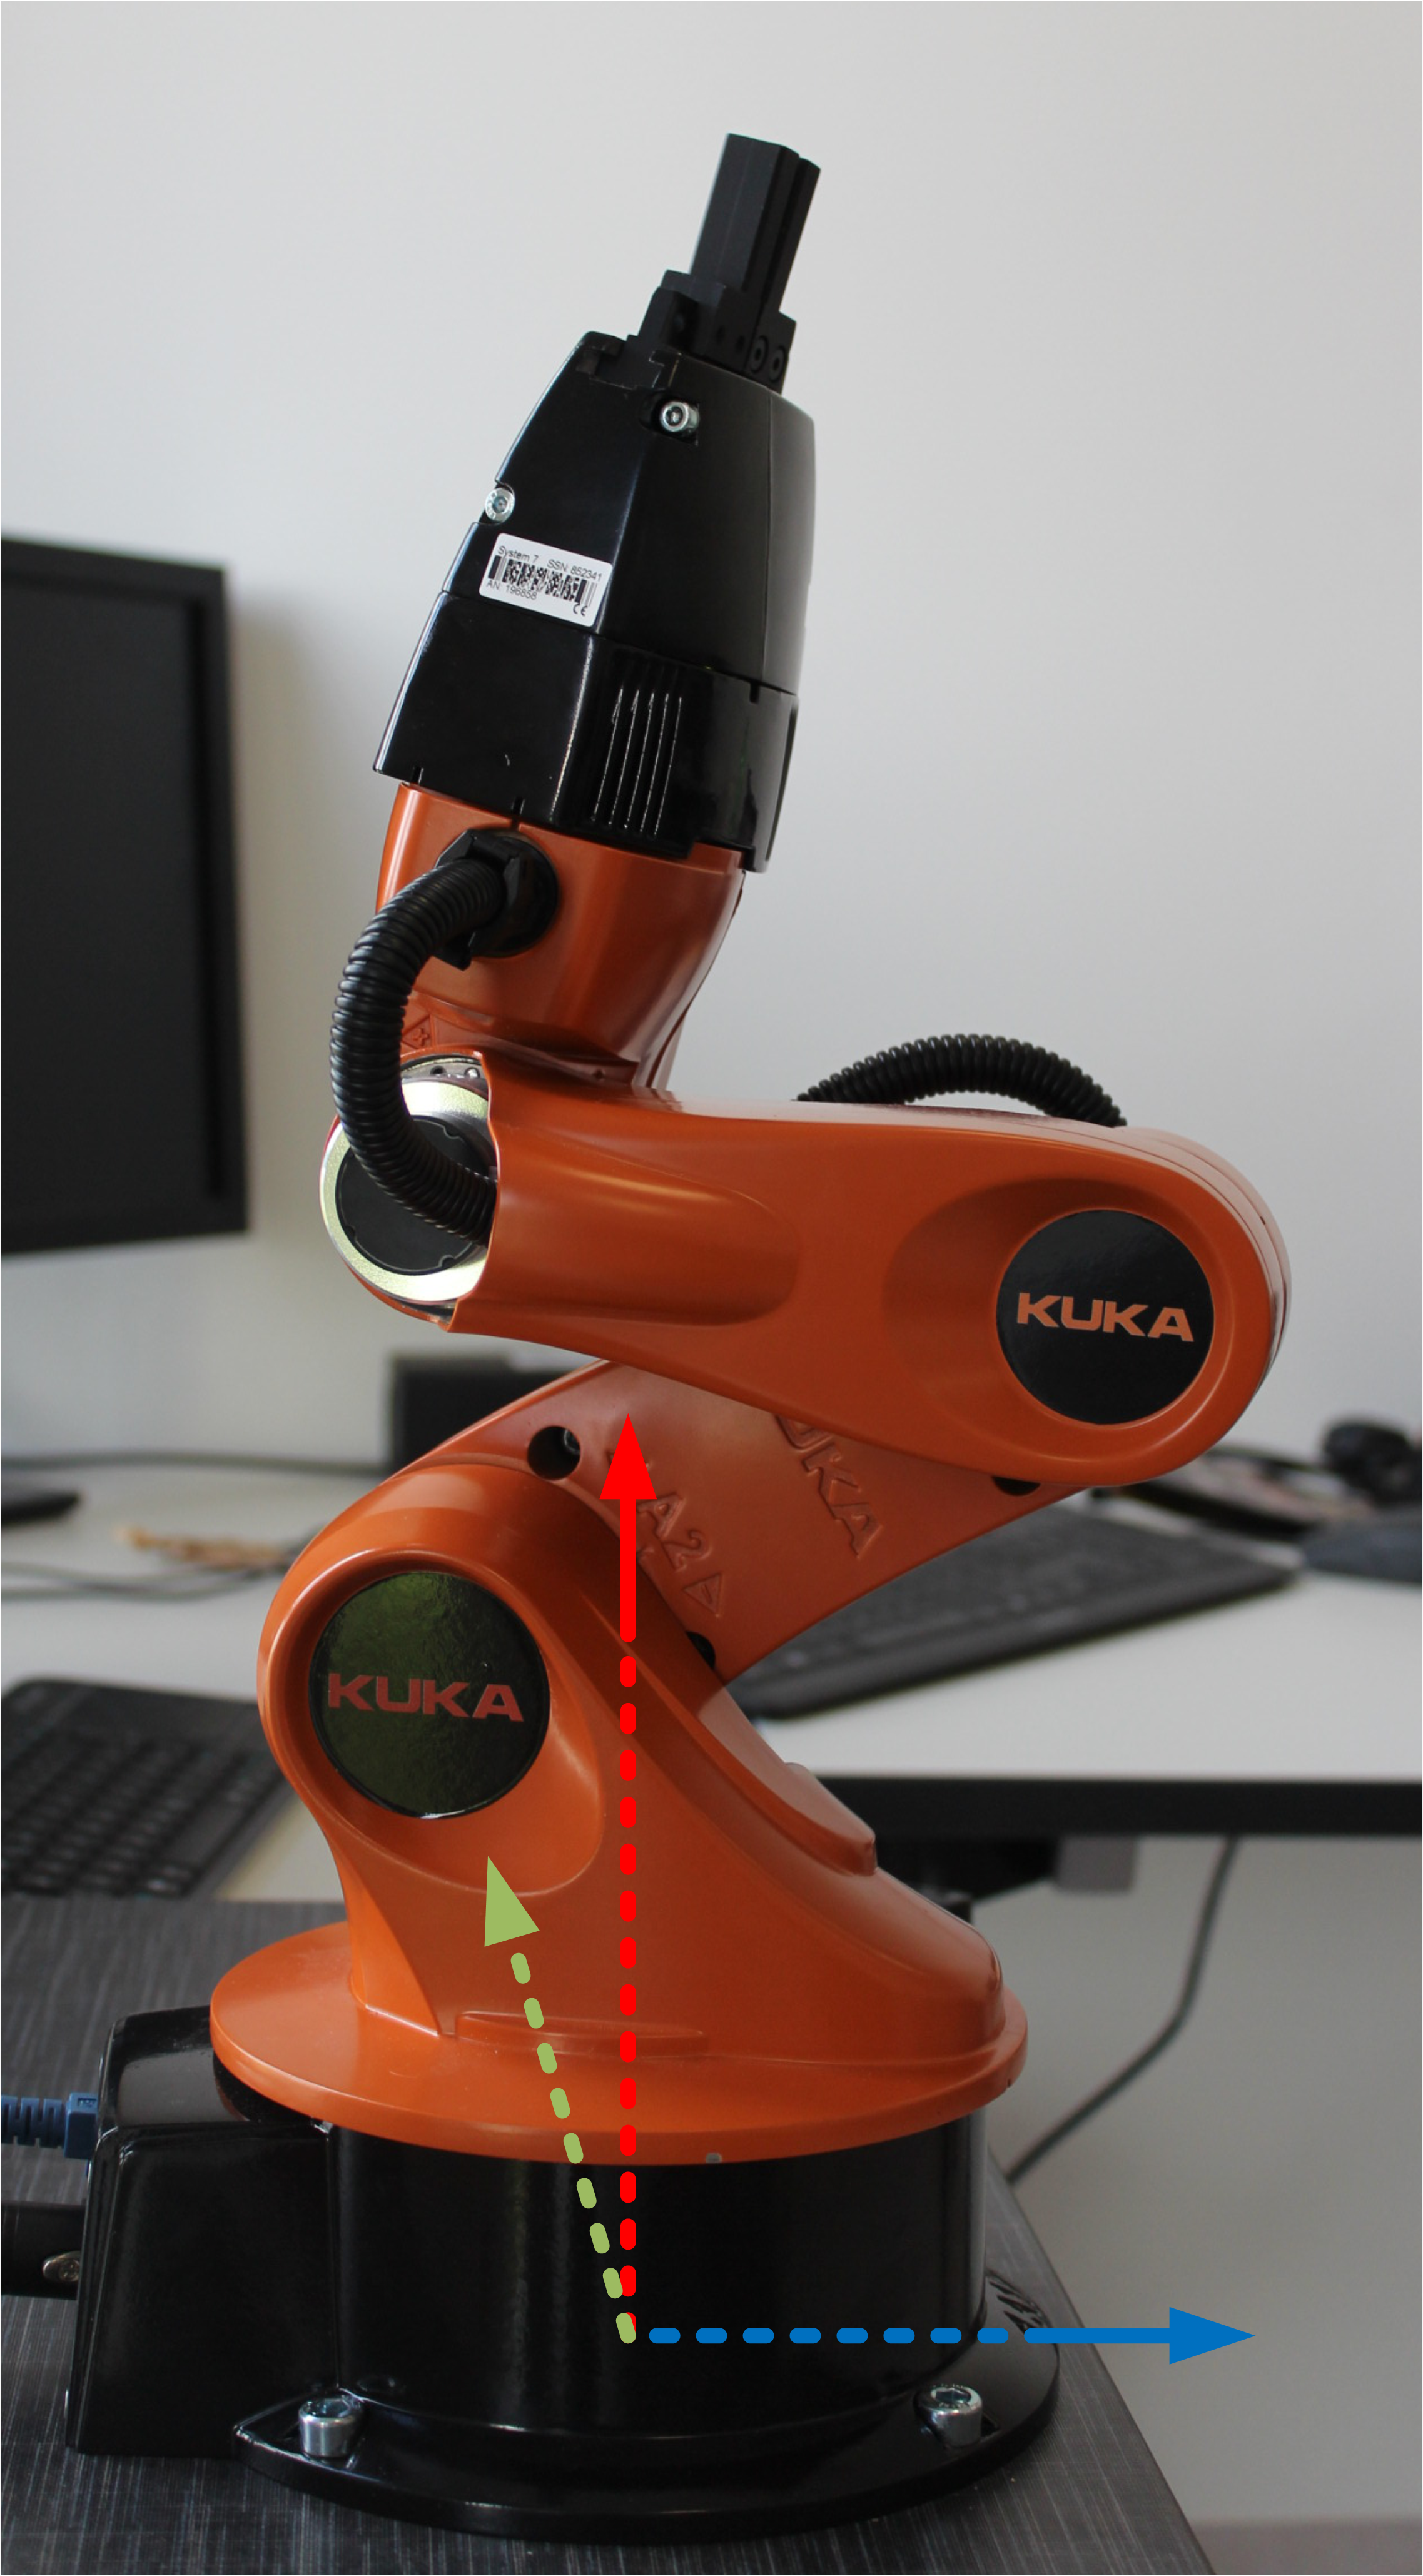
\includegraphics[scale=0.5]{fig/imgdummyk}
 		\label{fig:imgdummy}}
 	\hfill
 	\subfigure[Dummy und Rose in der Candle-Pose. Dummy ist auf dem Tisch montiert.]{%
 		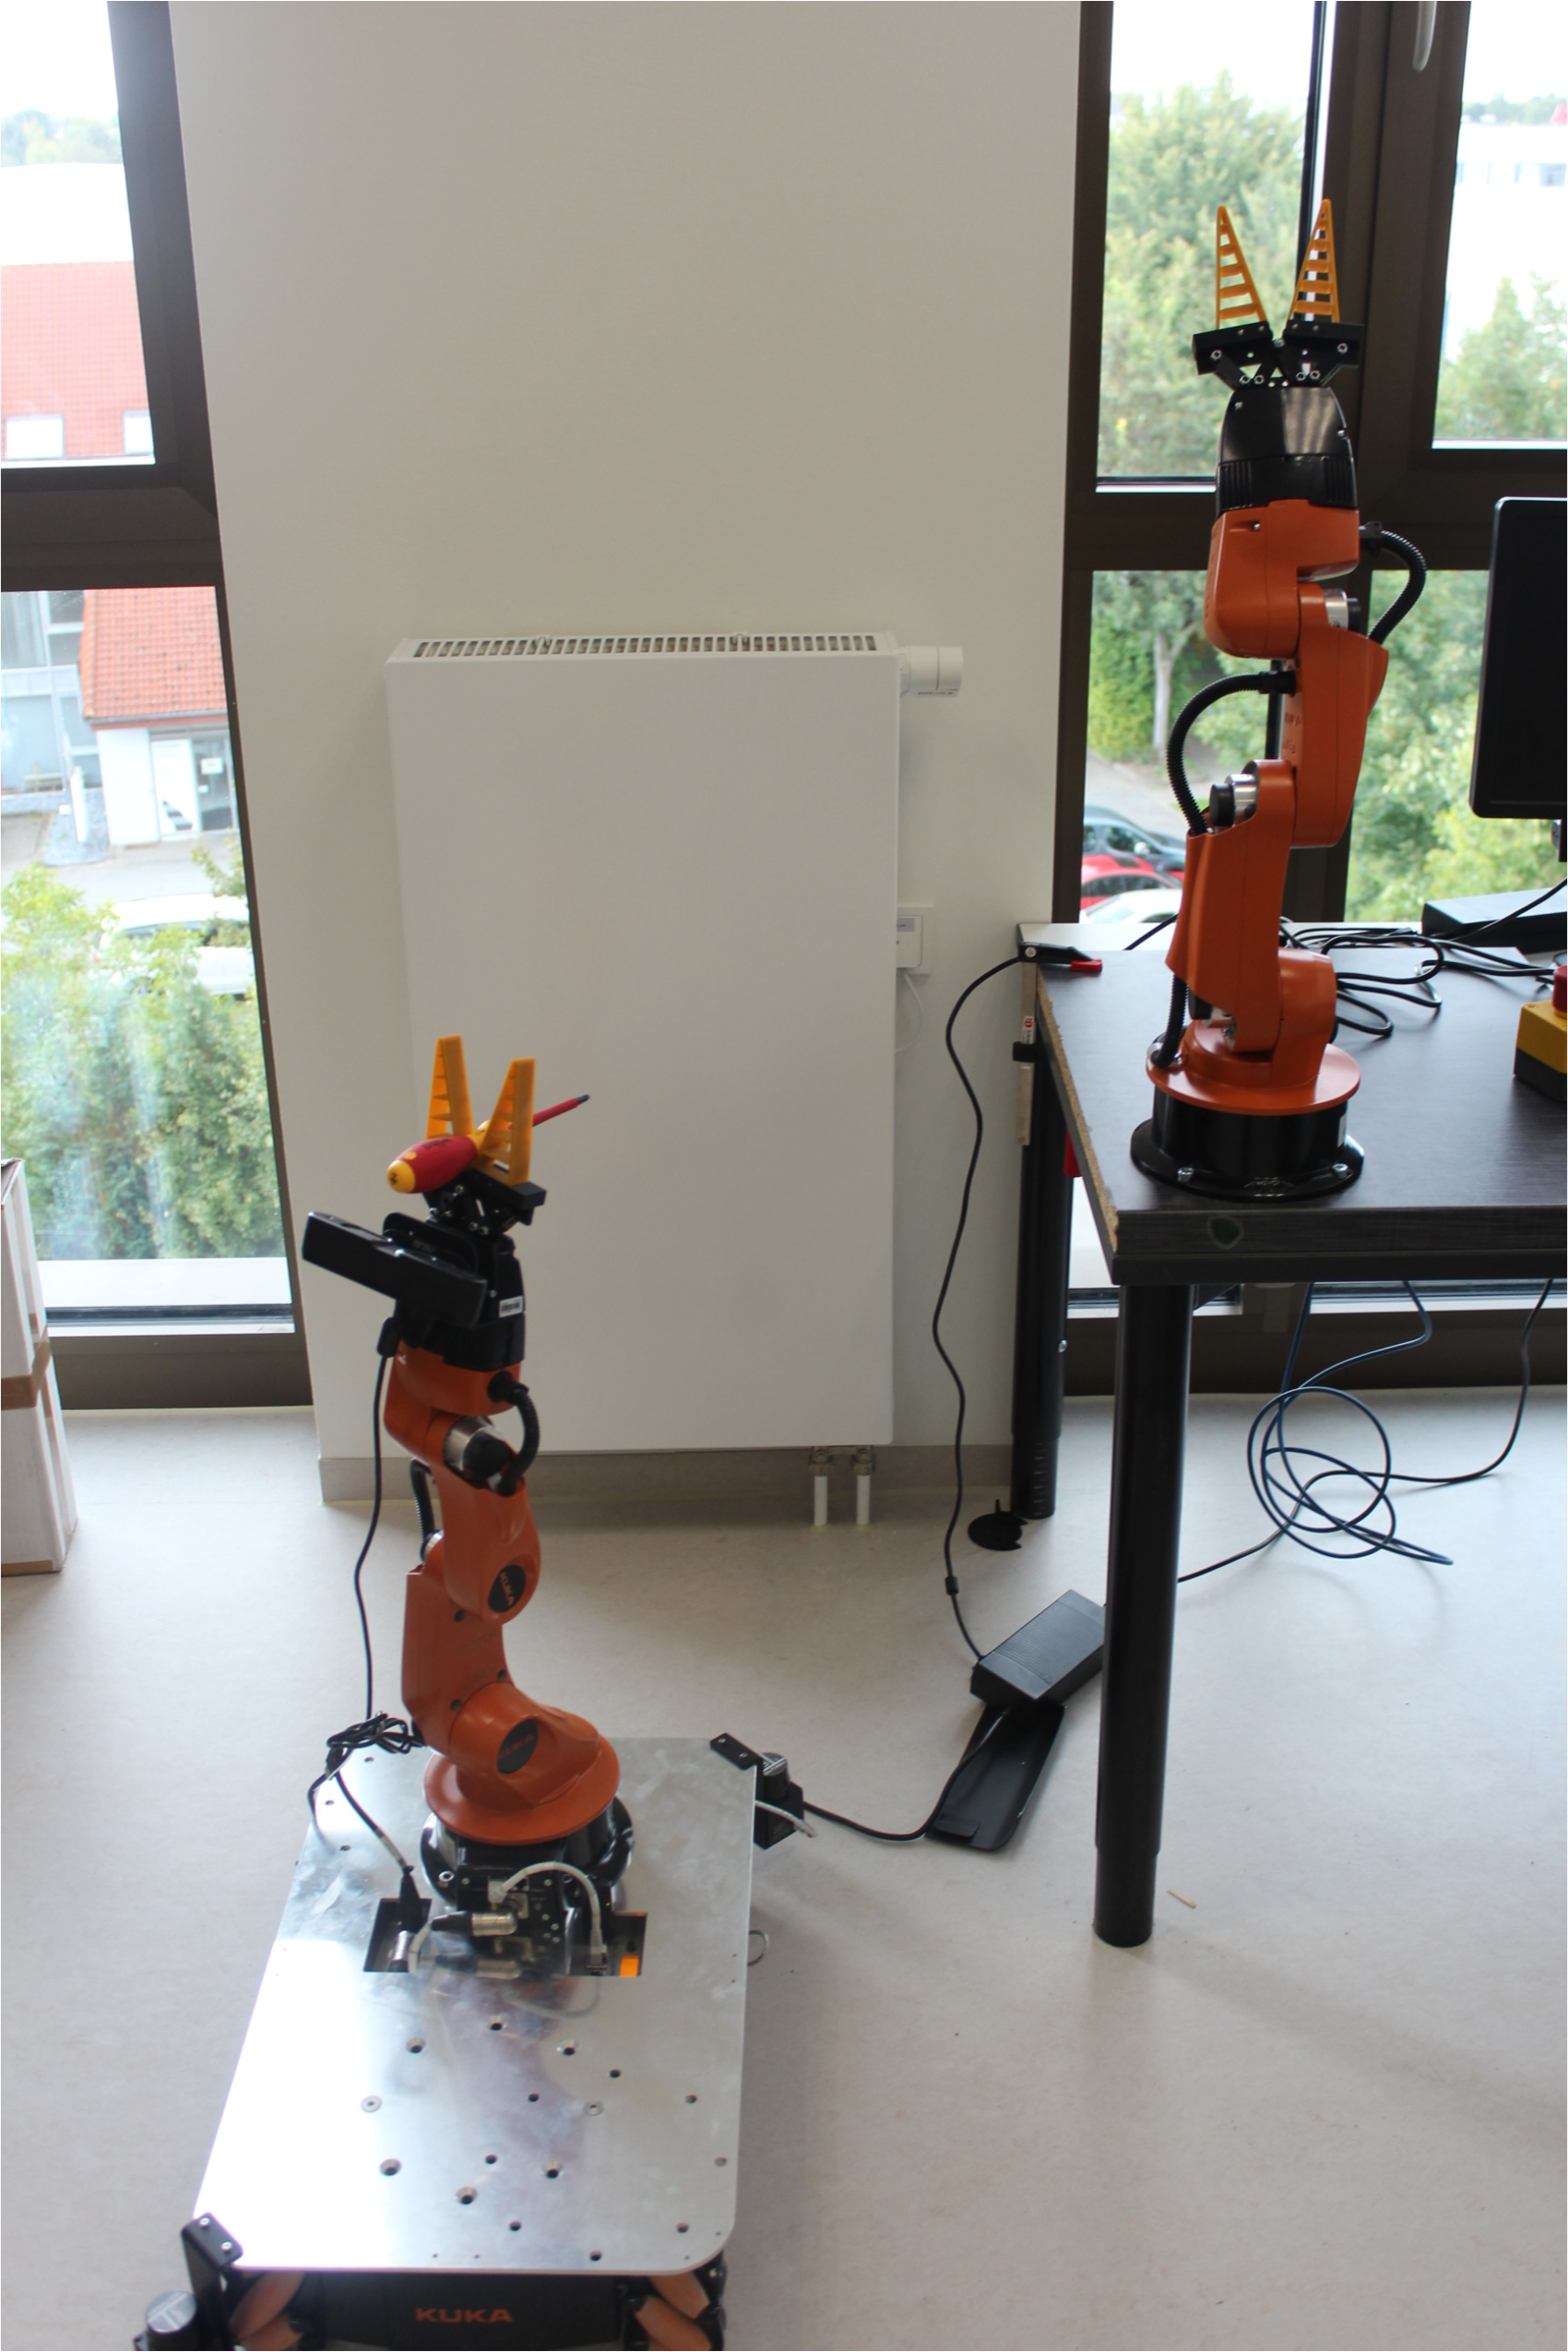
\includegraphics[scale=0.8]{fig/imgbothk}
 		\label{fig:imgboth}}
 	\caption{Fotografien der YouBots im Teststand}
 	\label{fig:img}
 \end{figure}


\subsubsection{Manipulator}
 Die Roboterarme von Dummy und Rose sind eine offene kinematische Kette mit fünf Gelenken, die von der Basis aufsteigend nummeriert sind. An Gelenk 5 sind die Greifer montiert. Diese bestehen aus zwei individuellen Fingern, die linear auf einer Achse bewegt werden können.

Gelenk 1 und Gelenk 5 sind zwei Drehgelenke um die Z-Achse. Diese liegen bei ausgestreckter Haltung (Candle-Pose) parallel. Gelenk 2, 3 und 4 sind Kippgelenke um die X-Achse, die immer parallel liegen. Durch diese Konstellation ergeben sich für den kompletten Arm fünf Freiheitsgrade (5-DOF). Durch die Einschränkung der Achsen auf die X- und Z-Achsen der einzelnen Gelenke ist ein seitlicher Griff bei $x_{base} = 0$ oder $y_{base} = 0$ nicht möglich. Die Höhe des Roboters in der Candle-Pose beträgt inklusiv Greifer 655 mm. Die einzelnen Abstände lassen sich der Grafik \ref{fig:basic-aufbau-youbot-kinematik} entnehmen.

\begin{figure}[H]
	\centering
	\includegraphics[scale=0.8]{fig/kukaarm_1}   
	\caption[YouBot Arm Kinematik]{YouBot Arm Kinematik. Links: Detailierter Mechanismus mit Gelenk und Glieder Angaben. Rechts: Vergrößerte Darstellung der Basis. Bildquelle: \cite{monikaflorekjasinska2015}}
	\label{fig:basic-aufbau-youbot-kinematik}
\end{figure}



 
 Tabelle \ref{tab:basic-aufbau-youbot-joints} stellt noch einmal den Drehbereich aller Gelenke dar. Dabei sind neben Bezeichner auch die minimalen und maximalen Winkel, sowie die Winkelgeschwindigkeiten enthalten. Eine Besonderheit stellt Gelenk 3 dar. Durch den Aufbau bedingt, wurde die Achse innerhalb der Treiber gespiegelt, sodass die Winkel um den 0° Punkt gespiegelt wurden. In der Tabelle und den folgenden Zeichnungen ist diese Spiegelung nicht beachtet.
 
   \begin{table}[H]
   	\begin{tabular}{|c|c|c|}
   		\hline Bezeichnung & Max./Min. Winkel & Winkelgeschwindigkeit (rad / s) \\ 
   		\hline Gelenk 1 & $\pm$ 2.94 & $\frac{\pi}{2}$  \\ 
   		\hline Gelenk 2 & + $\frac{\pi}{2}$ / -1.13  & $\frac{\pi}{2}$ \\ 
   		\hline Gelenk 3 & +2.54 /-2.63 & $\frac{\pi}{2}$ \\ 
   		\hline Gelenk 4 & $\pm$1.78 & $\frac{\pi}{2}$ \\ 
   		\hline Gelenk 5 & $\pm$2.91 & $\frac{\pi}{2}$ \\ 
   		\hline 
   	\end{tabular}
   	\caption[YouBot Arm Gelenke]{YouBot Arm Gelenke. Quelle: \cite{monikaflorekjasinska2015}}
   	\label{tab:basic-aufbau-youbot-joints}
   \end{table}
   
   Der Arbeitsraum des YouBot Arms beschränkt sich durch die Gelenke. Die Grafiken \ref{fig:basic-aufbau-youbot-workspace} und \ref{fig:basic-aufbau-youbot-workspace-top} stellen den Arbeitsbereich eingeschränkt dar. Die Darstellung \ref{fig:basic-aufbau-youbot-workspace} zeigt mit Hilfe von Konturen die einzelnen Bahnen unter Beschränkung der Gelenke, sowie der End-Effektor Ausrichtung.  Die äußere Kontur gibt die maximale Reichweite für den End-Effektor an. Die Z-Achse steht dabei orthogonal zur Tangente an der Konturposition. Abbildung \ref{fig:basic-aufbau-youbot-workspace-top} gibt eine Draufsicht auf den Arbeitsraum. Durch die Beschränkung von Gelenk 1 befindet sich ein toter Winkel im "Rücken" des Arms. Dieser kann durch einen Überschlag des ganzen Arms, insbesondere Gelenk 2 und 3, und einer 180 \textdegree Drehung von Gelenk 1 dennoch erreicht werden. Dies wird durch den linken Bereich in Abbildung \ref{fig:basic-aufbau-youbot-workspace} klar.
   
   \begin{figure}
   	\centering
   	\subfigure[YouBot Arm Arbeitsraum. Reichweite der einzelnen Gelenk und einzelne Abmessung der Links und Link-Offsets. Einheitslose Angaben sind in mm.]{%
   		\includegraphics[scale=0.55]{fig/kukaarm_2}
   		\label{fig:basic-aufbau-youbot-workspace}}
   	\hfill
   	\subfigure[Draufsicht YouBot Arm Arbeitsraum.]{%
   		\includegraphics[scale=0.55]{fig/kukaarm_3}
   		\label{fig:basic-aufbau-youbot-workspace-top}}
   	\caption{Arbeitsraum YouBot. Bilderquelle:\cite{monikaflorekjasinska2015}}
   	\label{fig:basic-aufbau-youbot-workspace-full}
   \end{figure}

\subsubsection{Mobile Plattform}
Rose besitzt neben dem Arm noch eine mobile Plattform. Diese ist 590 mm lang, 380 mm breit und 140 mm hoch. Die Plattform hat vier Räder mit einem Durchmesser von 47.5 mm. Jedes Rad lässt sich getrennt ansteuern. Bei den Rädern handelt es sich um Mecanum-Räder, die eine Steuerung in alle Richtungen ermöglichen. Dazu sitzen auf jeder Felge sechs drehbare tonnenförmige Rollen, die im Winkel von 45° zur Achse des Rades angebracht sind. Damit omni-direktionale Bewegungen möglich sind, werden die Räder abwechselnd zum Nachbar auf +45° oder -45° angeordnet. Die minimale Geschwindigkeit der Plattform beträgt $0.01\frac{m}{s}$, die maximale  $0.8\frac{m}{s}$. Abbildung \ref{fig:basic-aufbau-youbot-base} zeigt Aufbau und Abmessungen der Plattform. 

\begin{figure}[H]
	\centering
	\includegraphics[scale=0.8]{fig/kukabase}   
	\caption[YouBot Base]{YouBot Base. A = 74.87 mm, B = 100 mm, C = 471 mm, D = 300.46 mm E = 28 mm. Die Bodenfreiheit der Plattform beträgt 20 mm. Bildquelle: \cite{monikaflorekjasinska2015}}
	\label{fig:basic-aufbau-youbot-base}
\end{figure}

Die Plattform von Rose ist modifiziert und besitzt eine Aufsatzplatte. Diese dient zur Montage zusätzlicher Sensoren und zum Schutz der Räder bei Kollisionen. Diese ist 600 mm lang und 396 mm breit. Durch die Abstandsbolzen und die Dicke der Platte (5 mm) erhöht sich die Plattform auf 150 mm (siehe Abbildung \ref{fig:basic-aufbau-youbot-base_side}).  

 \begin{figure}[H]
 	\centering
 	\subfigure[Seitenansicht mobile Plattform mit Sensorplatte]{%
 		\includegraphics[scale=0.55]{fig/base2}
 		\label{fig:basic-aufbau-youbot-base_side}}
 	\subfigure[Draufsicht mobile Plattform mit Sensorplatte]{%
 		\includegraphics[scale=0.55]{fig/base3}
 		\label{fig:basic-aufbau-youbot-base-top}}
 	\caption{Mobile YouBot Plattform mit Sensorplatte. Bilderquelle: \cite{kuka2015}}
 	\label{fig:basic-aufbau-youbot-base-full}
 \end{figure}

\subsubsection{Rechner}
Für die Rechenleistung der beiden Roboter sorgen neben den verbauten, eingebetteten Boards zwei Computer mit Linux Betriebssystemen.
Der für Rose zuständige PC ist ein Mini-ITX und in der mobilen Plattform eingebaut. Dieser läuft mit einem Intel Atom D510 Dual Core mit 1.66 GHz als CPU und 2 GB DDR2 RAM. Als Festplattensystem ist eine 32 GB SSD verbaut. Der Rechner stellt einige IO-Schnittstellen zur Verfügung: sechs USB 2.0, ein VGA und zwei LAN Anschlüsse sind nutzbar. Dabei ist ein LAN Anschluss für den EtherCAT-Anschluss der Plattform belegt. Diese wiederum bringt nochmal zwei LAN Anschlüsse mit. Der Rechner für Dummy ist ein Dell Desktop-PC mit einem 3 GHz Dual Core Prozessor und 3 GB RAM. 

\subsection{Sensoren}
\label{sec:aufbau-sensoren}
Für die Erkennung von Objekten und der Positionierung im Raum sind mehrere Sensoren nötig. In dieser Arbeit wird dabei auf das Kamerasystem Asus XTion Pro Live und auf einen Laserscanner Hokuyo URG-04LX-UG01 zurückgegriffen.

\subsubsection{Asus XTion Pro}
Die XTion Pro ist ein Tiefenkamerasystem von Asus. Es besteht aus einer RGB-Kamera, einer Tiefen-Kamera und zwei Mikrophonen. Die Kamera wurde von Prime Sense entwickelt und ist eine umgelabelte Microsoft Kinect. Die XTion ist kleiner und leichter als die Kinect und damit besser für die Robotik geeignet. Angeschlossen wird die XTion mit einem USB Kabel und betrieben mit dem ROS Paket OpenNI2. Der Node published eine PointCloud mit RGB Daten, sowie eine PointCloud für die Tiefenkamera, als auch Bilder der RGB Kamera.

Das Sichtfeld der Kamera beträgt horizontal 58\textdegree, 45\textdegree vertikal und 70\textdegree diagonal. Die Auflösung der Tiefenkamera beträgt bei 30 Frames pro Sekunde 640x480 und bei 60 FPS 320x240. Die Auflösung des RGB-Bildes 1280x1024. Die nutzbare Distanz der Tiefenkamera beträgt zwischen 800 mm und 3500 mm.\cite{asus2015} Diese Distanz schränkt die Nutzbarkeit der Kamera ein, so ist sie nicht für eine visuelle Unterstützung der Greifer geeignet, wenn sie an diesen montiert ist, da die Distanz zwischen Kamera und Greifer kleiner 800 mm ist.

\begin{figure}[H]
	\centering
	\includegraphics[scale=0.8]{fig/xtion1}   
	\caption[Asus Xtion Pro Live]{Asus XTion Pro Live. Bildquelle: \cite{asus2015}}
	\label{fig:aufbau-xtion}
\end{figure}

\subsubsection{Hokuyo URG-04LX-UG01}
Der URG-04LX-UG01 ist ein optischer Abstandsmesser. Dieser kann Entfernungen in einer zirkulären Ebene messen. Entwickelt wurde er von der Firma Hokuyo, welche neben dem URG noch weitere, ähnliche Sensoren anbietet, die andere Reichweiten und Sichtfelder abdecken. Die Sensoren nutzen zur Messung der Entfernung eine Infrarot-Diode mit einer Wellenlänge von 785 nm. Die Distanz wird mit Hilfe der Phasenverschiebung berechnet. Diese Technik reduziert den Einfluss durch das Oberflächenmaterial des gemessenen Objektes. Versorgt wird der Sensor mit 5V DC, welche über den USB-Anschluss angelegt werden. Da die Startleistung des Sensors die maximale Abgabeleistung eines einzigen USB-Anschluss überschreitet, müssen ein Y-USB-Kabel und zwei USB-Anschlüsse genutzt werden. Angesteuert wird der Sensor mit dem ROS-Paket Hokuyo-Node, welche eine PointCloud published.

Der URG-Sensor hat eine Reichweite von maximal 4000 mm und benötigt für eine Messung 100 ms, was einer Messrate von 10 FPS entspricht. Das Sichtfeld beträgt 240\textdegree. Die minimale Graduelle Auflösung beträgt 0.36\textdegree. Dadurch ergeben sich die ungefähren Disparitäten von 20 mm bei 2000 mm und maximal 40 mm bei 4000 mm Radius. Die Ungenauigkeit beträgt maximal 3 Prozent des gemessenen Wertes, was bei der maximalen Reichweite von 4000 mm einer Abweichung von 120 mm entspricht.\cite{maeda2009}

 \begin{figure}[H]
 	\centering
 	\subfigure[Produktbild. Bildquelle: \cite{nowak2015}]{%
 		\includegraphics[scale=2.5]{fig/hok2}
 		\label{fig:aufbau-hok2}}
 	\subfigure[Schema: Reichweite und Sichtfeld. Sichtfeld in Messpunktsektoren (MP) unterteilt. Verändert nach: \cite{maeda2009}]{%
 		\includegraphics[scale=0.7]{fig/hok1}
 		\label{fig:aufbau-hok1}}
 	\caption{Hokuyo URG-04LX-UG01}
 	\label{fig:aufbau-hok}
 \end{figure}

\subsubsection{Argos 3D - P100}
Ein weiterer Tiefensensor ist die Argos 3D – P100 von Bluetechnix. Diese arbeitet mit dem Time of Flight (ToF) Prinzip. Der Sensor wird mit einem USB-Kabel angesteuert, benötigt aber noch eine weitere Stromzufuhr. Der Sensor kann aus ROS mit einem eigenen Node angesprochen werden. Der Sensor hat eine Reichweite zwischen 100 mm und 3000mm. Die Framerate beträgt bis zu 160 FPS bei ein Auflösung von 160 x120. Das Sichtfeld beträgt 90 \textdegree.\citep{bluetechnix2015}

\begin{figure}[H]
	\centering
	\includegraphics[scale=0.8]{fig/argos3d}   
	\caption[Argos 3D - P100]{Argos 3D - P100. Bildquelle: \cite{bluetechnix2015}}
	\label{fig:aufbau-argos3d}
\end{figure}

\subsection{Koordinatensysteme}
Im Verlauf dieser Arbeit werden häufig rechtshändige kartesische Koordinatensysteme genutzt. Unterschieden wird vor allem zwischen dem globalen und den lokalen Koordinatensystemen. Das globale Koordinatensystem bezieht sich auf den Teststand. Der Ursprung liegt dabei in Ecke der Wände auf dem Boden. Die positive Z-Achse zeigt dabei nach oben und die positive X-Achse liegt entlang der Fensterreihe. Dadurch zeigt die positive Y-Achse von der Fensterwand weg. Die lokalen Koordinatensysteme sind immer von ihrem Kontext abhängig. So besitzen zum Beispiel die YouBot Arme, die Greifer und die mobile Plattform eigene Koordinatensysteme. Diese sind meistens voneinander abhängig. Bei den YouBot Arme zeigt die positive Z-Achse von der Grundfläche zu dem ersten Gelenk. Die positive X-Achse zeigt vom Ursprung zur \textit{A1}-Markierung, welche gegenüber den Anschlüssen liegt (siehe Abbildung \ref{fig:imgdummy}). Der Ursprung liegt im Mittelpunkt der Grundfläche des Arms. Bei der mobilen Plattform liegt der Ursprung in der Mitte der Sensorplatte. Die positive Z-Achse zeigt nach oben und die positive X-Achse nach vorne zur KUKA Aufschrift. Alle lokalen Koordinatensysteme haben einen Bezug zum globalen Koordinatensystem. Dieser besteht aus einer Translation und einer Rotation.

\subsection{Netzwerk- und Sensoranbindung}

\begin{figure}[H]
	\centering
	\includegraphics[scale=0.5]{fig/netw}   
	\caption[Schematische Darstellung der Verbindungen]{Schematische Darstellung der Verbindungen}
	\label{fig:aufbau-netw}
\end{figure}

Abbildung \ref{fig:aufbau-netw} stellt den genutzten Verbindungsplan dar. Die zentrale Komponente ist der Router, welcher mit einem externen Access-Point (AP) eine WLAN-Verbindung ermöglicht. Mit diesem WLAN verbinden sich die beiden Steuerungsrechner \textit{Rose} und \textit{Dummy}, welche beide unter diesen Hostnames im Netz erreichbar sind. Die Verbindungen auf beiden Seiten sind gleich gehalten. Die Verbindung zwischen Rechner und Roboter sind mit der EtherCAT-Schnittstelle (Ethernet for Control Automation Technology) realisiert. Diese Ethernet-Variante wurde für Echtzeit-Anforderungen entwickelt, indem Wert auf kurze Zykluszeiten ($\leq$ 100 $\mu$s) und  niedrigem Jitter für exakte Synchronisierung ($\leq$ 1 $\mu$s) gelegt wurde \citep{ethercat}.  Die Verbindung zwischen den Rechnern und den Sensoren ist mit USB-Verbindungen umgesetzt. Dabei werden alle USB-Anschlüsse auf der mobilen Plattform von Rose vollständig durch die Sensoren, sowie dem WLAN-USB-Dongle und dem Tastatur/Maus-Dongle belegt. Weitere USB-Geräte sind nur durch einen zusätzlichen HUB möglich. 

Eine Alternative zu diesem Plan ist ein vermaschtes Netz, wie bei PEIS gefordert. Dadurch könnte der Router wegfallen, da alle Endgeräte direkt miteinander verbunden sind. Des Weiteren könnten einige Sensoren auf eigene Rechner ausgegliedert werden. Dies würde die einzelnen Rechner, besonders den leistungsschwachen Rechner von Rose, entlasten, aber auch die Netzwerkkomplexität und die Kosten steigern.

\clearpage



%%%%%%%%%%%%%%%%%%%%%%%%%%%%%%%%%%%%%%%%%%%%%%%%%%%%%%%%%%%%%%%%%%%%%%%
%% Inhaltliche Kapitel
% TODO anpassen
%%%%%%%%%%%%%%%%%%%%%%%%%%%%%%%%%%%%%%%%%%%%%%%%%%%%%%%%%%%%%%%%%%%%%%%%
%% Inhaltliches Kapitel (Beispiel)
\section{Beispiel für Inhalte}
\label{sec:content}

Dieses Kapitel ist als Beispiel für die zu erstellenden Inhalte gedacht.



\subsection{Nutzung von Aufzählungen}
    \subsubsection{Einfache Aufzählungen}
        Einfache Aufzählungen erhält man über die \texttt{Itemize}-Umgebung:
        \begin{itemize}
        	\item erster Stichpunkt
        	\item zweiter Stichpunkt
            \begin{itemize}
            	\item erster verschachtelter Stichpunkt
            	\item noch einer
            	\begin{itemize}
            		\item Schachteln auf dritter Ebene
        		\end{itemize}
        	\end{itemize}
        	\item dritter Stichpunkt
        \end{itemize}
        
    \subsubsection{Nummerierte Aufzählungen}
        Aufzählungen lassen sich auch automatisch durchnummerieren mit der
        \texttt{Enumerate}-Umgebung:
        \begin{enumerate}
            \item erster Stichpunkt
            \item zweiter Stichpunkt
            \begin{itemize}
                \item erster verschachtelter Stichpunkt
                \item noch einer
                \begin{itemize}
                    \item Schachteln auf dritter Ebene
                \end{itemize}
            \end{itemize}
            \item dritter Stichpunkt
        \end{enumerate}
        
    \subsubsection{Definitions-Aufzählungen}
        Mit der \texttt{Description}-Umgebung lassen sich Definitions-artige Aufzählungen
        gestalten.
        \begin{description}
            \item[Begriff] und hier die längliche Beschreibung des tollen Begriffs,
            seiner Auswirkungen auf den Geisteszustand des Schreibers und die Folgen für
            den Leser
            \item[B2] noch ein Begriff
        \end{description}
    
    
    
\subsection{Tabellen und Bilder}
    \subsubsection{Einbinden von Abbildungen}
        Einfache Abbildungen lassen sich mit der \texttt{Figure}-Umgebung und dem
        \texttt{includegraphics}-Befehl einbinden:
        \begin{figure}
            \centering
            \includegraphics[scale=1.4]{fig/exampleSzene}   
            \caption{Typischer Beispieltext}
            \label{fig:beispielText}
        \end{figure}
            
        Abbildungen mit mehreren Teilabbildungen lassen sich über die
        \texttt{Subfigure}-Umgebung nutzen.
        \begin{figure}
            \centering
            \subfigure[teil 1]{%
                \includegraphics[scale=1]{fig/exampleSzene}
                \label{fig:beispielDepiktionenA}}
            \hfill
            \subfigure[teil 2]{%
                \includegraphics[scale=1]{fig/exampleSzene}
                \label{fig:beispielDepiktionenB}}
            \vfill
            \subfigure[teil 3]{%
                \includegraphics[scale=1]{fig/exampleSzene}
                \label{fig:beispielDepiktionenC}}
            \caption{Zum Beispieltext passende Abbildungen (Depiktionen)}
            \label{fig:beispielDepiktionen}
        \end{figure}
        
        Als Quellen eigenen sich PDF- und JPG-Dateien. Andere Dateien müssen vor der
        Benutzung konvertiert werden.
    
    
    \subsubsection{Tabellen}
        Tabellen gehen in der \texttt{Table}-Umgebung mit Hilfe des \texttt{tabular}-Befehls.
        \begin{table}
            \centering
            \begin{tabular}{l|l||r}
                \multicolumn{2}{l}{zwei Spalten zusammengefasst} & dritte Spalte\\
                Spalte 1 & Spalte 2 & Spalte 3 \\\hline\hline
                Spalte 1 & Spalte 2 & Spalte 3 \\\hline
                Spalte 1 & Spalte 2 & Spalte 3 \\\hline
            \end{tabular}
            \caption{Beispieltabelle}
            \label{tab:beispieltabelle}
        \end{table}
        
        Ansonsten funktioniert die Umgebung änhlich wie die
        \texttt{Figure}-Umgebung.
    
    
    \subsubsection{Quellcode}
        Quellcode lässt sich mit Hilfe des \texttt{Listings}-Paketes einbinden.
        Sinnvollerweise definiert man sich dazu in der Präambel des
        Hauptdokuments eine passende neue \texttt{lstnewenvironment}-Umgebung, die man
        dann einfach nutzen kann und die neben Snytax-Highlighting auch andere
        Dinge wie Rahmen, Zeilennummern, Bildunter- oder überschriften
        etc.~beherrscht.
        
        \begin{figure}
        \centering
        \begin{java}
public class Student {
    private String name;

    public Student(String name) {
        this.name = name; 
    }
    
    public static void main(String[] args) {
        Student s = new Student();
    }
}
        \end{java}
        \caption{Sourcecode für Kram}
        \label{fig:source}
        \end{figure}
        
        
     \subsubsection{Quellcode}
        Algorithmen schreibt man entweder als Pseudocode (über das
        \texttt{Listings}-Paket) oder aber mit Hilfe der \texttt{algorithm}-Umgebung aus
        dem Paket \texttt{algorithm2e}
        
        \begin{center}
        \begin{algorithm}[ht]
        \DontPrintSemicolon
        \LinesNumbered
        \SetKwFunction{init}{init}
        \SetKwFunction{evaluate}{evaluate}
        \SetKwFunction{recombine}{recombine}
        \SetKwFunction{mutate}{mutate}
        \SetKwFunction{select}{select}
        \SetKw{nicht}{not}
        \SetKw{und}{and}
        \Begin{
            $t$ = 0\;
            \init{$P(t)$}\;
            \evaluate{$P(t)$}\;
            \While{\nicht optimal \und \nicht Abbruch}{
                $PP(t) = $ \recombine{$P(t)$}\;
                \mutate{$PP(t)$}\;
                \evaluate{$PP(t)$}\;
                $P(t+1) = $ \select{$PP(t)$, $P(t)$}\;
                $t = t+1$\;
            }
        }
        \caption{Ablauf eines hybriden EA}
        \label{alg:eaHybrid}
        \end{algorithm}
        \end{center}
        

    
\subsection{Referenzierungen}
    \subsubsection{Zitate}
    Zitieren geht mit dem Befehl \texttt{cite}: \cite{Claus98a} bzw. mit den Befehl
    \texttt{citep}: \citep{wagner2009tele}. Als Argument
    benötigt man den Schlüssel für die jeweilige Referenz, so wie er in der
    .bib-Datei hinterlegt ist bzw.~durch Tools wie JabRef generiert wird. 
    
    Wenn man etwas nicht direkt zitieren möchte, aber die Literaturquelle im
    Literaturverzeichnis erscheinen soll, dann nutzt man den Befehl
    \texttt{nocite}.
    
    \subsubsection{Querverweise}
    Den Anker für die Querverweise setzt man mit dem Befehl \texttt{label}.
    Bezugnehmen kann man dann mit Hilfe von \texttt{ref} oder \texttt{pageref},
    wobei ersteres durch die entsprechende Gliederungsnummer (Überschrift,
    Abbildung, Tabelle, \ldots) ersetzt wird und letzteres durch die
    Seitennummer, auf der der Anker für die Referenz gesetzt wurde.
    Beispiel: Abbildung \ref{fig:beispielText} erscheint auf Seite
    \pageref{fig:beispielText}.
    
    
\subsection{Fussnoten}
    Fussnoten setzt man mit Hilfe des Befehls \texttt{footnote}. Dieser folgt
    entweder direkt auf das Wort, welches man mit einer Fussnote versehen möchte
    oder aber auf das Satzendezeichen, wenn man einen ganzen Satz/Absatz meint.
    Beispiel:\footnote{Das ist meine erste Fussnote.}
    
    
\subsection{Mathe}
Für Mathe siehe \href{http://www.ams.org/tex/short-math-guide.html}{{\tt
www.ams.org/tex/short-math-guide.html}}.


    
    
    
\clearpage
%%%%%%%%%%%%%%%%%%%%%%%%%%%%%%%%%%%%%%%%%%%%%%%%%%%%%%%%%%%%%%%%%%%%%%%




%%%%%%%%%%%%%%%%%%%%%%%%%%%%%%%%%%%%%%%%%%%%%%%%%%%%%%%%%%%%%%%%%%%%%%%
%% Zusammenfassung und Ausblick
%%%%%%%%%%%%%%%%%%%%%%%%%%%%%%%%%%%%%%%%%%%%%%%%%%%%%%%%%%%%%%%%%%%%%%%
%% Zusammenfassung und Ausblick
\section{Zusammenfassung und Ausblick}
Dieses Kapitel bildet den Abschluss dieser Arbeit.  Neben einer Zusammenfassung wird ein Ausblick über mögliche Weiterentwicklungen und Verbesserungen gegeben. Dabei wird auf die analysierten Schwachstellen des Systems eingegangen.

\subsection{Zusammenfassung}
In dieser Arbeit wurde ein Multi-Robot-System entwickelt. Dieses nutzt weitere Aktoren und Sensoren, ähnlich einem intelligenten Gebäude, zur Interaktion mit der Umwelt. Zentrale Komponenten dieses Systems sind zwei Roboter. Beide Robotersysteme bestehen aus einem Roboterarm. Der eine Roboter besitzt zudem eine mobilen Plattform, eine 3D-Kamera und einen Lasersensor. Als Anwendungsszenario wurde die Aufnahme durch den mobilen Roboter und die Übergabe an den stationären Roboter implementiert. Dabei wurden 3D-Kameras zur Objekterkennung und -Lokalisierung genutzt. Die Implementierung dafür nutzt Algorithmen aus der Computer Vision, genauer aus der Punktwolken Verarbeitung. Die dabei erreichte Genauigkeit der Sensoren und Algorithmen beträgt fünf Zentimeter bei der Raumüberwachung und fünf Millimeter bei der Nahfelderkennung. 

Zur effizienten Steuerung der Arme wurde iterativ eine eigene inverse Kinematik entwickelt. Diese beruht auf geometrischen Grundsätzen. Bei Tests zeigten diese eine Genauigkeit von circa vier Millimetern von den linearen und 0,6 Grad für den rotierenden Anteil der Zielpose. Für die Bewegung auf einer Trajektorie wurde ein Ansatz gewählt, der mit Hilfe von Wegpunkten den Ausschlag des Greifers verhindert. Nicht genau untersucht wurde die Entwicklung einer genauen Navigation der mobilen Plattform. Aus Gründen der Priorität wurde diese nur sehr rudimentär entwickelt. Bedingt durch ungenaue Odometriedaten bei Bewegungen entlang der Y-Achse kommt es zu hohen Ungenauigkeiten. Auch der Einsatz von Lasersensoren kann diesem nur bedingt entgegenwirken, da diese abhängig von einem Referenzpunkt der Odometrie sind. Andere Ansätze, wie SLAM, sind dabei viel genauer.

 Bei der Entwicklung des MRS wurde auf bestehenden Arbeiten, wie der PEIS-Ökologie, aufgebaut. Neben den Robotern kamen auch weitere eigenständige Sensoren und Aktoren zum Einsatz. RATS erweitert PEIS um die Möglichkeit für parallele und komplexere Koordinierung. Diese kann auch unter den einzelnen Agenten innerhalb eines RATS stattfinden. Da in dieser Arbeit die Anzahl an Robotern, Aktoren und Sensoren sehr gering ist, wurde die Konfiguration des MRS statisch implementiert. Eine Schnittstelle für eine dynamische Konfiguration ist im Konzept für RATS jedoch vorgesehen.

In dieser Arbeit konnte aus Platzgründen nicht auf weitere erarbeitete Konzepte eingegangen werden. Die Grundlagen für diese beruhen auf dieser Arbeit. Auch die Implementierung wurde im Rahmen dieser Arbeit durchgeführt. Dazu gehören Problematiken um den Greifer, der in dieser schriftlichen Ausarbeitung nur am Rande betrachtet wurde. Auf Grund mangelnder Griffigkeit des Greifer zum starren Testobjekt, kam es zum Einsatz des pinken Radiergummis. Dieses weißt einen hohen Reibungskoeffizienten und eine weiche, sowie flexible Struktur auf. Außerdem war es anhand der Farbe leicht zu identifizieren. Ein weiterer Randaspekt ist die Einbindung eines weiteren Aktors in das RATS-System. Dazu wurde im Rahmen dieser Arbeit eine farbige Lichtanlage installiert und implementiert, die dem Anwender oder anderen Personen im Labor ein visuelles Feedback über den Zustand des Robotersystems gibt.

\subsection{Ausblick}
\label{sec:ausblick}
Da der Umfang dieser Arbeit begrenzt ist, konnten nicht alle Ideen umgesetzt werden und wurden einigen Stellen angemerkt. Diese Ideen befassen sich mit der Erweiterbarkeit, aber auch mit der Verbesserung des Systems. Grundlegende Ansätze sind dabei der Greifer, die Koordinierung und Konfigurierung, die Autonomie des MRS und vor allem die Navigation, beziehungsweise Lokalisierung.

Der Greifer vom YouBot besteht aus zwei parallelen Fingern. Durch deren harte und glatte Beschaffenheit ist der Greifen von vielen Gegenständen nicht möglich. Auch die Erweiterung mit Softgrippern ließ keinen vernünftigen Griff zu. Eine erste Erweiterungsmöglichkeit stellt ein Greifer mit drei Fingern in Bogenform dar. Diese ermöglichen auch das Greifen von runden und kleinen Gegenständen. Die zweite Alternative besteht aus einem Greifer der aus einem Ballon, gefüllt mit feinkörnigem Granulat, besteht. Dieses umschließt das Zielobjekt und bildet bei Unterdruck eine feste Struktur, die das Objekt festhält. TODO Quelle

Für die Koordinierung und Konfigurierung existieren viele Arbeiten. Für das RATS empfiehlt sich eine Auktionsstruktur für das dynamische Zuweisen der Aufgaben, wie in TODO. Auch die Konfigurierung sollte einem dynamischen Ansatz folgen, damit zentrale Elemente wie der RATSCore entfallen können. Außerdem ist eine Umstellung von einem Router auf ein gemaschtes Netzwerk sinnvoll. Damit neue Agenten beitreten oder alte sich entfernen können. Eine Selbstbewertung des Systems und die automatische Anpassung von Konfigurationsparametern ist eine Möglichkeit die Autonomie des Systems zu erhöhen.

Alternativen für die Navigation und Lokalisierung gibt es viele. So ist ein Umstieg auf eine funkbasierte Lokalisierung, vergleichbar wie GPS, möglich. Auch Bild-basierte Ansätze, zum Beispiel durch die Raumüberwachung, sind denkbar. Am sinnvollsten ist vermutlich jedoch das SLAM-Verfahren, da vorhandene Lasersensoren genutzt werden können. Dieses würde die Genauigkeit des Systems stark steigern und damit auch eine Überarbeitung einzelner Konzepte ermöglichen.


\clearpage


%%%%%%%%%%%%%%%%%%%%%%%%%%%%%%%%%%%%%%%%%%%%%%%%%%%%%%%%%%%%%%%%%%%%%%%
%% Danksagung
%%%%%%%%%%%%%%%%%%%%%%%%%%%%%%%%%%%%%%%%%%%%%%%%%%%%%%%%%%%%%%%%%%%%%%%
%% Danksagung
\section{Danksagung}

    % TODO anpassen
    Ich bin allen Leuten furchtbar dankbar, vor allem den Jungs bei Google.


\clearpage


%%%%%%%%%%%%%%%%%%%%%%%%%%%%%%%%%%%%%%%%%%%%%%%%%%%%%%%%%%%%%%%%%%%%%%%
%% Literatur
%% braucht einen Zwischenlauf mit "bibtex abschlussarbeit"
%% nach Änderungen: pdflatex, bibtex, pdflatex, pdflatex, pdflatex
%%%%%%%%%%%%%%%%%%%%%%%%%%%%%%%%%%%%%%%%%%%%%%%%%%%%%%%%%%%%%%%%%%%%%%%
%% Literatur
\section{Literaturverzeichnis}
\label{sec:literatur}

    \bibliography{babib}    % braucht einen Zwischenlauf mit "bibtex abschlussarbeit"
    \bibliographystyle{plainnat}
%    \bibliographystyle{alpha}   % normales bibtex; [abk.nam+jahr]
%     \bibliographystyle{alphadin}   % bibtex nach DIN [abk.nam+jahr]
%     \bibliographystyle{babalpha}  % bibtex mit babelbib
%     \bibliographystyle{chicago} % (name, jahr)
%     \bibliographystyle{splncs}  % nur (1)
%     \bibliographystyle{named}
    
    
%     TODO anpassen
    % diese hier zusätzlich auf alle Faelle ins Literaturverzeichnis
    \nocite{}

    
    
    \clearpage


%%%%%%%%%%%%%%%%%%%%%%%%%%%%%%%%%%%%%%%%%%%%%%%%%%%%%%%%%%%%%%%%%%%%%%%
%% Anhang
%%%%%%%%%%%%%%%%%%%%%%%%%%%%%%%%%%%%%%%%%%%%%%%%%%%%%%%%%%%%%%%%%%%%%%%
%% Anhang
\begin{appendix}
    
        \section{Testdaten MoveIt Bewegungsplaner}
        \label{app:tmv}
        
    \begin{table}[H]
    	\centering
    	\begin{tabular}{|c|c|c|c|}
    		\hline  	& EST & PRM & CHOMP \\ 
    		\hline 10 	& 
    		$\left(\begin{array}{c} 1.84 \\ 6.253 \\ 11.6  \end{array}\right)$ & 
    		$\left(\begin{array}{c} 0.32 \\ 10.486 \\ 17.4  \end{array}\right)$ &
    		$\left(\begin{array}{c} 0.46 \\ 11.731 \\ 13.2  \end{array}\right)$ \\ 
    		\hline 100 	&
    		$\left(\begin{array}{c} 15.84 \\ 2.214 \\ 2.1  \end{array}\right)$ & 
    		$\left(\begin{array}{c} 3.84 \\ 3.164 \\ 4.6  \end{array}\right)$ &
    		$\left(\begin{array}{c} 5.21 \\ 4.756 \\ 2.9  \end{array}\right)$ \\ 
    		\hline 1000 &  
    		OOT &
    		$\left(\begin{array}{c} 36.15 \\ 1.54 \\ 1.2  \end{array}\right)$ &
    		$\left(\begin{array}{c} 40.84 \\ 1.78 \\ 0.8  \end{array}\right)$ \\ 
    		\hline 
    	\end{tabular}
    	
    	\caption[Gemittelte Messwerte der MoveIt!-Planer-Algorithmen]{Die gemittelten Messwerte der MoveIt!-Planer. In den Zeilen sind die unterschiedlichen Iterationen pro Planung gegeben. Die Spalten geben den verwendeten Planer-Algorithmus an. Die Messwerte $x$ setzen sich aus der benötigten Planungszeit $x_1$ in Sekunden und der euklidischen Distanz der Zielpose zur Planpose zusammen. Dabei wird zwischen linearer $x_2$ (Zentimeter) und rotierender $x_3$ (Grad) Distanz unterschieden. OOT steht für eine Überschreitung der Zeitschranke bei allen Bewegungszielen.}
    	
    	\label{tab:mesplan}
    \end{table}
    
    
        \section{Testdaten Inverse Kinematik}
    \label{app:tdik}
    
    \begin{tabular}{|c|c|c|}
    	\hline
    	Pose&Diff Lin in cm&Diff Rot in \textdegree \\
    	    	\hline
    	1&0,0431&0,4581\\
    	    	\hline
    	2&0,2226&0,1110\\
    	    	\hline
    	3&0,3716&0,0594\\
    	    	\hline
    	4&0,0341&0,3559\\
    	    	\hline
    	5&0,1523&0,6661\\
    	    	\hline
    	6&0,0380&0,1763\\    	\hline
    	7&0,0970&0,6651\\    	\hline
    	8&0,1287&0,6553\\    	\hline
    	9&0,3358&0,1190\\    	\hline
    	10&0,0310&0,6070\\    	\hline
    	11&0,0327&0,3736\\    	\hline
    	12&0,0847&0,3640\\    	\hline
    	13&0,3369&0,3008\\    	\hline
    	14&0,1834&0,4781\\    	\hline
    	15&0,0294&0,1417\\    	\hline
    	16&0,3784&0,2441\\    	\hline
    	17&0,2717&0,1017\\    	\hline
    	18&0,1019&0,4557\\    	\hline
    	19&0,1778&0,1373\\    	\hline
    	20&0,2016&0,4597\\    	\hline
    	21&0,2314&0,1427\\    	\hline
    	22&0,0504&0,1256\\    	\hline
    	23&0,1733&0,5850\\    	\hline
    	24&0,0187&0,2859\\    	\hline
    	25&0,1995&0,5118\\    	\hline
    	\\    	\hline
    	Mittelwerte&0,1570&0,3432\\    	\hline
    	Max&0,3784&0,6661\\    	\hline
    	Min&0,0187&0,0594\\    	\hline
    	
    	
    \end{tabular} 
    
    \section{Messwerte Systemtest}
    \label{app:systest}
    \begin{center}
    	\begin{longtable}{|c|c|c|c|c|c|c|c|}
    		\hline
    		Testlauf & Äquivalenzklasse &$\gamma$ & $\eta$ & $k$ & $j$ & $\iota$ & Erfolg oder Fehler\\
    		\hline
    		\hline
    		1 & X-Kurz & $\left(\begin{array}{c} 2,2 \\ 1,6\end{array}\right)$ & $\left(\begin{array}{c} 3,2 \\ -0,4\end{array}\right)$ & $0$ & $2$ & <1cm& \checkmark\\
    		\hline
    		2 & X-Kurz &  $\left(\begin{array}{c} -2,1 \\ 1,3\end{array}\right)$ & $\left(\begin{array}{c} 4,1 \\ -0,3\end{array}\right)$ & 0 & 4 & <1cm & \checkmark\\
    		\hline
    		3 & X-Kurz &  $\left(\begin{array}{c} 1,4 \\ 2,2\end{array}\right)$ & $\left(\begin{array}{c} 3,5 \\ -0,5\end{array}\right)$ & 0 & 2& <1cm& \checkmark\\
    		\hline
    		4 & X-Kurz &  $\left(\begin{array}{c} 2,3 \\ -2,1\end{array}\right)$ & $\left(\begin{array}{c} 3,7 \\ -0,3\end{array}\right)$ & 0& 2&<1cm & \checkmark\\
    		\hline
    		5 & X-Lang &  $\left(\begin{array}{c} -1,6 \\ 1,8\end{array}\right)$ & $\left(\begin{array}{c} 5,2 \\ -0,7\end{array}\right)$ & 1& 2& <1cm& \checkmark\\
    		\hline
    		6 & X-Lang &  $\left(\begin{array}{c} 1,4 \\ 1,4\end{array}\right)$ & $\left(\begin{array}{c} 6,1 \\ -0,8\end{array}\right)$ & 1& 3& <1cm& \checkmark\\
    		\hline
    		7 & X-Lang &  $\left(\begin{array}{c} 1,3 \\ -2,2\end{array}\right)$ & $\left(\begin{array}{c} 7,2 \\ -0,8\end{array}\right)$ & 0& 2& <1cm& \checkmark\\
    		\hline
    		8 & X-Lang &  $\left(\begin{array}{c} 5,4 \\ 1,3\end{array}\right)$ & $\left(\begin{array}{c} 6,8 \\ -0,5\end{array}\right)$ & 1& 2& <1cm& \checkmark\\
    		\hline
    		9 & X-Kurz, Y-Kurz &  $\left(\begin{array}{c} 2,1 \\ -1,5\end{array}\right)$ & $\left(\begin{array}{c} 10,4 \\ -4,8\end{array}\right)$ & >10& -& -& Fehler 1\\
    		\hline
    		10 & X-Kurz, Y-Kurz &  $\left(\begin{array}{c} 1,2 \\ 3,8\end{array}\right)$ & $\left(\begin{array}{c} 4,2 \\ -7,4\end{array}\right)$ & 1& 3& <1cm& \checkmark\\
    		\hline
    		11 & X-Kurz, Y-Kurz &  $\left(\begin{array}{c} -2,4 \\ 4,2\end{array}\right)$ & $\left(\begin{array}{c} 3,7 \\ -6,3\end{array}\right)$ & 2& 4& <1cm& \checkmark\\
    		\hline
    		12 & X-Kurz, Y-Kurz &  $\left(\begin{array}{c} -3,2 \\ -2,1\end{array}\right)$ & $\left(\begin{array}{c} 6,1 \\ -4,2\end{array}\right)$ & 1& 2& 3,2& Fehler 3\\
    		\hline
    		13 & X-Lang, Y-Kurz &  $\left(\begin{array}{c} -4,1 \\ -2,8\end{array}\right)$ & $\left(\begin{array}{c} 3,8 \\ -7,2\end{array}\right)$ & 1& 3& 4,2& Fehler 3\\
    		\hline
    		14 & X-Lang, Y-Kurz &  $\left(\begin{array}{c} 7,2 \\ 1,2\end{array}\right)$ & $\left(\begin{array}{c} 9,4 \\ -4,8\end{array}\right)$ & 2& 4& 4,5& Fehler 3\\
    		\hline
    		15 & X-Lang, Y-Kurz &  $\left(\begin{array}{c} -1,4 \\ 8,1\end{array}\right)$ & $\left(\begin{array}{c} 6,2 \\ -5,5\end{array}\right)$ & 2& 3& <1cm& \checkmark\\
    		\hline
    		16 & X-Lang, Y-Kurz &  $\left(\begin{array}{c} 2,4 \\ 1,3\end{array}\right)$ & $\left(\begin{array}{c} -1,2 \\ -4,2\end{array}\right)$ & 2& 3& <1cm& \checkmark\\
    		\hline
    		17 & X-Kurz, Y-Lang &  $\left(\begin{array}{c} 1,2 \\ -3,4\end{array}\right)$ & $\left(\begin{array}{c} 5,4 \\ -22,8\end{array}\right)$ & >10& -&- & Fehler 1\\
    		\hline
    		18 & X-Kurz, Y-Lang &  $\left(\begin{array}{c} 3,8 \\ 2,1\end{array}\right)$ & $\left(\begin{array}{c} 3,2 \\ -17,2\end{array}\right)$ & 2& >10& -& Fehler 2\\
    		\hline
    		19 & X-Kurz, Y-Lang &  $\left(\begin{array}{c} 2,5 \\ 2,4\end{array}\right)$ & $\left(\begin{array}{c} 1,6 \\ -20,1\end{array}\right)$ & 1& 7& <1cm& \checkmark\\
    		\hline
    		20 & X-Kurz, Y-Lang &  $\left(\begin{array}{c} 1,6 \\ 2,7\end{array}\right)$ & $\left(\begin{array}{c} 4,2 \\ -19,8\end{array}\right)$ & 2& 8& 4,2cm& Fehler 3\\
    		\hline
    		21 & X-Lang, Y-Lang &  $\left(\begin{array}{c} 3,2 \\ -1,7\end{array}\right)$ & $\left(\begin{array}{c} 3,8 \\ -21,2\end{array}\right)$ & 1& 6& 5,6cm& Fehler 3\\
    		\hline
    		22 & X-Lang, Y-Lang &  $\left(\begin{array}{c} 2,4 \\ 2,1\end{array}\right)$ & $\left(\begin{array}{c} 2,8 \\ -18,4\end{array}\right)$ & 2& 5& <1cm& \checkmark\\
    		\hline
    		23 & X-Lang, Y-Lang &  $\left(\begin{array}{c} -3,3 \\ 1,6\end{array}\right)$ & $\left(\begin{array}{c} 2,8 \\ -31,4\end{array}\right)$ & >10& -& -& Fehler 1\\
    		\hline
    		24 & X-Lang, Y-Lang &  $\left(\begin{array}{c} 2,7 \\ 1,8\end{array}\right)$ & $\left(\begin{array}{c} 3,1 \\ -16,1\end{array}\right)$ & 2& 8& 6,2& Fehler 3\\
    		\hline
    		\caption{Messwerte der Testphase}
    		\label{tab:messw}
    	\end{longtable}
    \end{center}
    
\end{appendix}


\clearpage








%%%%%%%%%%%%%%%%%%%%%%%%%%%%%%%%%%%%%%%%%%%%%%%%%%%%%%%%%%%%%%%%%%%%%%%
%% Game over ;-)
\end{document}


